\documentclass[aspectratio=169,xcolor=dvipsnames]{beamer}
\usetheme{SimplePlus}

% Math
\usepackage{nicefrac}

% Tipography stuff
\usepackage{booktabs} % Allows the use of \toprule, \midrule and \bottomrule in tables
\usepackage[english]{babel}
\usepackage{csquotes}
\usepackage{microtype}
\usepackage{pdfpages}
\usepackage{fontawesome5}
\usepackage{soul}
\usepackage{euler}
\usepackage[linesnumbered]{algorithm2e}
\usepackage{animate}
\usepackage{ifthen}
\usepackage{multirow}

% Bibliography
\usepackage[giveninits,style=authoryear-comp,backend=biber]{biblatex}
\addbibresource{../fracbiblio.bib}
\newcommand\unnumbered{\setbeamertemplate{footline}{}}%\addtocounter{framenumber}{-1}
\renewcommand*{\bibfont}{\normalfont\small}

% Figures
\usepackage{tikz,pgfplots}
\usetikzlibrary{calc,arrows,patterns,matrix,external}
\usepackage{subfig}
\usepackage{graphicx} % Allows including images
\usepackage[american]{circuitikz}
\usepackage{tikz-network}
\tikzexternalize[prefix=Figures/] % activate and define figures/ as cache folder
\usepackage{mathtools}
\usepackage{pgfplotstable}

% Links
\usepackage{hyperref}
\hypersetup{colorlinks,linkcolor=,urlcolor=MidnightBlue}

% Code
\usepackage{minted}

% Block matrices
\newcommand{\bigzero}{\mbox{\normalfont\Large\bfseries 0}}
\newcommand{\rvline}{\hspace*{-\arraycolsep}\vline\hspace*{-\arraycolsep}}
\newcommand{\R}{\mathbb{R}}
\newcommand{\bone}{{\bf 1}}
\newcommand{\evec}{{\bf e}}
\newcommand{\dvec}{{\bf d}}
\newcommand{\xvec}{{\bf x}}
\newcommand{\yvec}{{\bf y}}
\newcommand{\qvec}{{\bf q}}
\newcommand{\svec}{{\bf s}}
\newcommand{\pvec}{{\bf p}}
\newcommand{\tvec}{{\bf t}}
\definecolor{Ao}{rgb}{0.0, 0.5, 0.0}
\setlength{\tabcolsep}{0.3em}


\author{Fabio Durastante}
\title{An introduction to fractional calculus}
\subtitle{Fundamental ideas and numerics}
\institute{Università di Pisa\\\href{mailto:fabio.durastante@unipi.it}{\faEnvelope\;fabio.durastante@unipi.it}\\\href{https://fdurastante.github.io}{\faFirefox\;fdurastante.github.io}}
\date{October, 2022}

\newcommand{\de}{{\rm d}}


\begin{document}
	
	{\unnumbered
		\begin{frame}[t,plain,noframenumbering]
			\titlepage
			\vspace{-4em}
\includegraphics[width=2cm]{frame.png}
		\end{frame}
	}

	\section{Variable coefficients cases}

	\begin{frame}{Variable coefficients cases}
	
	We now want to solve the \emph{slightly} more complex case
	\begin{equation*}
		\begin{cases}\frac{\partial W}{\partial t} = \alert{d^+(x,t)} \,{}^{\only<1->{RL}}D_{[0,x]}^\alpha W(x,t) + \alert{d^-(x,t)} {}^{\only<1->{RL}}D_{[x,1]}^\alpha W(x,t),\\
			W(0,t) = W(1,t) = 0, \qquad W(x,t) = W_0(x).	
		\end{cases}
	\end{equation*}
	with $d^{+}(x,t),d^{-}(x,t) \geq 0$ and \textbf{not identically} zero.
	\begin{enumerate}
		\item<2-> We go through all the \textbf{same discretization procedure}: from Riemann--Liouville to (shifted) Gr\"unwald--Letnikov, then series truncation, \emph{etc.}
		\item<3-> we obtain a matrix sequence of the form
		\[
		A_N = \nu I_N - \left( D_N^+ G_N + D_N^- G_N^T \right),
		\]
		where $D_N^{\pm}$ are \textbf{diagonal matrices} whose entries \textbf{sample the functions} $d^{\pm}_N(x,t)$ on the finite difference grid.
		\item[\faBomb]<4-> We \alert{\textbf{no longer have Toeplitz matrices}}!
	\end{enumerate}

	\end{frame}

	\begin{frame}{Not all hope is lost}
	
	\begin{itemize}
		\item[\faFastForward] We can still perform \textbf{fast matrix-vector products}:
		\[A_N \mathbf{x} = \nu \mathbf{x} - D_N^+ ( G_N \mathbf{x})  - D_N^- (G_N^T \mathbf{x})\]
		still $O(N \log N)$ cost.
		\item[{\faLightbulb[regular]}] Maybe we can use some \alert{trick} to reuse \alert{circulant preconditioners}
		\begin{enumerate}
			\item \normalsize If $d^{\pm}_N(x,t)$ do not vary much maybe we can \textbf{average them}, i.e.,
			\[
			P(t) = \nu I - \hat{d^+}(t) s(G_N) - \hat{d^-}(t) s(G_N^T),
			\]
			with $\hat{d^{\pm}}(t) = \nicefrac{1}{N} \sum_{i=1}^{N} d^{\pm}(x_i,t)$
		\end{enumerate}
	\end{itemize}
	
	\end{frame}

	\begin{frame}[fragile]{The averaging trick}
	Does it work?
	\[
	d^+(x,t) = \Gamma(3-\alpha)x^\alpha, \qquad d^-(x,t) = \Gamma(3-\alpha) (2-x)^\alpha 
	\]
\begin{onlyenv}<1>
\vspace{-3em}\definecolor{bg}{rgb}{0.95,0.95,0.95}%
\begin{minted}[bgcolor=bg,fontsize=\small,breaklines]{matlab}
w0 = @(x) 5*x.*(1-x);
hN = 1/(N-1); x = 0:hN:1; dt = hN; t = 0:dt:1;
dplus = @(x,t) gamma(3-alpha).*x.^alpha;
dminus = @(x,t) gamma(3-alpha).*(2-x).^alpha;
% Discretize
G = glmatrix(N,alpha); Gr = G; Grt = G.'; I = eye(N,N);
Dplus = diag(dplus(x,0)); Dminus = diag(dminus(x,0));
% Left-hand side
nu = hN^alpha/dt;
A = nu*I - (Dplus*Gr + Dminus*Grt);
\end{minted}
\end{onlyenv}
\begin{onlyenv}<2>
\vspace{-3em}\definecolor{bg}{rgb}{0.95,0.95,0.95}%
\begin{minted}[bgcolor=bg,fontsize=\small,breaklines]{matlab}
% Solve
[ev,evt] = sunprec(N,alpha);
c = nu + mean(dplus(x,0))*ev + mean(dminus(x,0))*evt;
P = @(x) cprec(c,x);
[X,FLAGsun,RELRESsun,ITERsun,RESVECsun] = gmres(A,(nu*w),[],1e-9,N,P);
\end{minted}
\end{onlyenv}
\only<3->{\vspace{-1.5em}
\begin{columns}
\begin{column}{0.25\columnwidth}
\begin{tabular}{llcl}
\toprule
$\alpha$ & $N$ & GMRES & P \\
\midrule
\multirow{7}{*}{1.2} & $2^{5}$ & 31 & 13 \\
& $2^{6}$ & 50 & 14 \\
& $2^{7}$ & 64 & 14 \\
& $2^{8}$ & 75 & 15 \\
& $2^{9}$ & 84 & 15 \\
& $2^{10}$ & 91 & 14 \\
& $2^{11}$ & 96 & 14 \\
\bottomrule
\end{tabular}
\end{column}

\begin{column}{0.25\columnwidth}
\begin{tabular}{llcl}
\toprule
$\alpha$ & $N$ & GMRES & P \\
\midrule
\multirow{7}{*}{1.4} & $2^{5}$ & 31 & 13 \\
& $2^{6}$ & 59 & 14 \\
& $2^{7}$ & 92 & 15 \\
& $2^{8}$ & 127 & 15 \\
& $2^{9}$ & 161 & 15 \\
& $2^{10}$ & 196 & 15 \\
& $2^{11}$ & 231 & 15 \\
\bottomrule
\end{tabular}
\end{column}

\begin{column}{0.25\columnwidth}
\begin{tabular}{llcl}
\toprule
$\alpha$ & $N$ & GMRES & P \\
\midrule
\multirow{7}{*}{1.6} & $2^{5}$ & 32 & 13 \\
& $2^{6}$ & 62 & 13 \\
& $2^{7}$ & 112 & 14 \\
& $2^{8}$ & 183 & 14 \\
& $2^{9}$ & 262 & 14 \\
& $2^{10}$ & 353 & 14 \\
& $2^{11}$ & 456 & 14 \\
\bottomrule
\end{tabular}
\end{column}

\begin{column}{0.25\columnwidth}
\begin{tabular}{llcl}
\toprule
$\alpha$ & $N$ & GMRES & P \\
\midrule
\multirow{7}{*}{1.8} & $2^{5}$ & 32 & 12 \\
& $2^{6}$ & 64 & 12 \\
& $2^{7}$ & 126 & 13 \\
& $2^{8}$ & 225 & 13 \\
& $2^{9}$ & 378 & 13 \\
& $2^{10}$ & 559 & 12 \\
& $2^{11}$ & 779 & 12 \\
\bottomrule
\end{tabular}
		\end{column}
		
\end{columns}}

\only<4>{\vspace{1em}\faWrench\, We have \textbf{doubled the number of iterations} but things still seem reasonable$\ldots$}
	\end{frame}

\begin{frame}{Can we prove anything?}\vspace{-1em}
What did we actually prove for the \emph{constant coefficient case}?
\begin{itemize}
	\only<2,3>{\item[\faCog]<2-> We computed the \textbf{asymptotic spectral distribution} of the matrix sequence $\{\nu A_N\}_N$ (\emph{eigenvalues} for the symmetric case, \emph{singular values} for the general case);}
	\item[\faCog]<3-> We proved that $P^{-1} A_N - I = $``small norm''$+$``small rank'', i.e., that the preconditioner delivered a \textbf{clustering of the eigenvalues}.
\end{itemize} 
\begin{columns}
\begin{column}{0.5\columnwidth}\centering
\only<4,5>{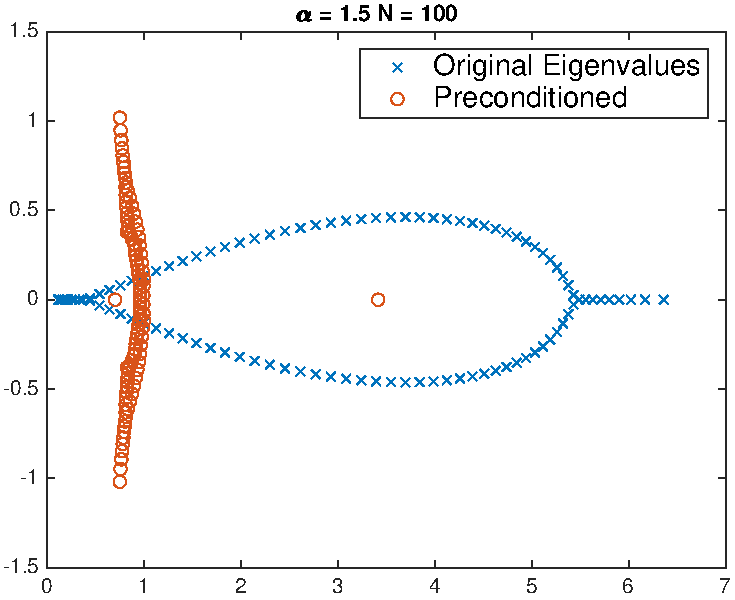
\includegraphics[width=0.7\columnwidth]{ev15_100.pdf}}%
\only<6->{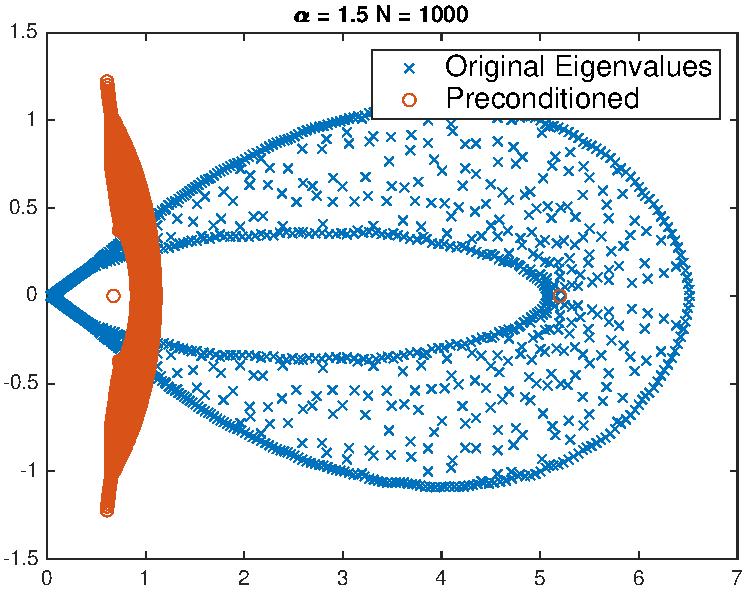
\includegraphics[width=0.7\columnwidth]{ev15_1000.pdf}}%
\end{column}
\begin{column}{0.5\columnwidth}\centering
\only<5,6>{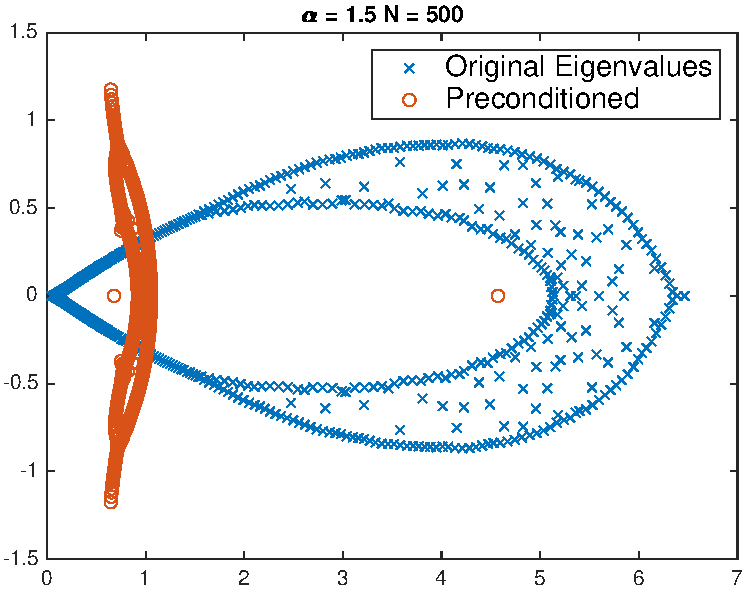
\includegraphics[width=0.7\columnwidth]{ev15_500.pdf}}%
\only<7->{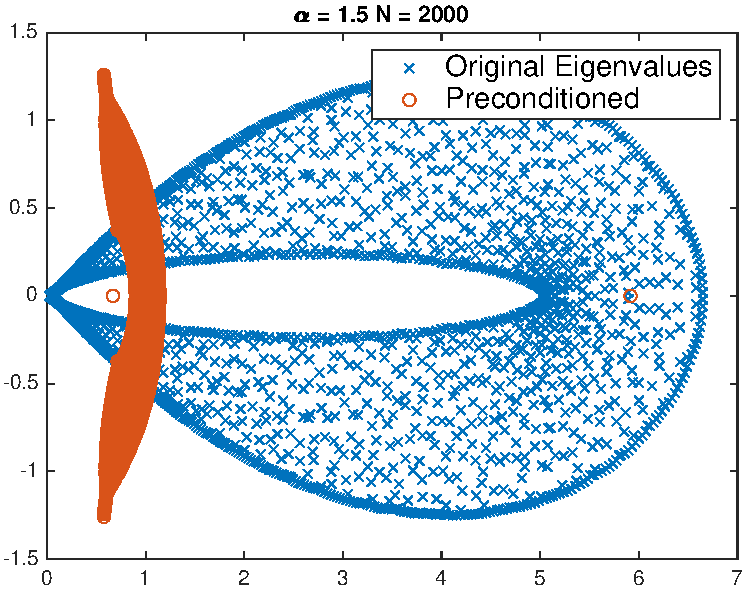
\includegraphics[width=0.7\columnwidth]{ev15_2000.pdf}}%
\end{column}
\end{columns}

\onslide<8->{\alert{\faEye} We \textbf{don't have a cluster}, yet eigenvalues are in a fairly small region.}

\onslide<9->{\alert{\faGlasses}\;let's investigate!}

\end{frame}

\begin{frame}{Having a cluster: $C_n - A_n$}
	
	For two matrix sequences $\{C_n\}_n$ and $\{A_n\}_{n}$ (both of order $n$) we say that they are \alert{$\varepsilon$-close} by rank if
	\begin{equation}\tag{$\varepsilon$-close}\label{eq:rankeps}
		\forall\,\varepsilon > 0 \; A_n - C_n = E_{n,\varepsilon} + R_{n,\varepsilon}, \quad \begin{array}{l}\|E_{n,\varepsilon}\|_2 \leq \varepsilon, \\ \operatorname{rank}(R_{n,\varepsilon}) \leq r(n,\varepsilon) = o(n) \text{ for } n \rightarrow +\infty,\end{array}
	\end{equation}
	\begin{itemize}
		\item[\faCogs]<2-> Let $\gamma_n(\varepsilon)$ count how many singular values $\sigma(A_n - C_n)$ are greater than $\varepsilon$, i.e.,
		\[
		\gamma_n(\varepsilon) = \left\lvert\{ j \,:\, \sigma_j(A_n - C_n) > \varepsilon, \quad j=1,\ldots,n \}\right\rvert,
		\]
		\item[$\Rightarrow$]<3-> \eqref{eq:rankeps} is telling us that $\gamma_n(\varepsilon) = o(n)$ for $n \rightarrow + \infty$.
		\item[\faLightbulb]<4-> Then we know that $\{A_n - C_n\}_n$ has a singular value \textbf{cluster} at zero, if $\gamma_n(\varepsilon) = O(1)$ which holds equally with $r(n,\varepsilon) = r(\varepsilon) = O(1)$ for any $\varepsilon > 0$ then we have a \textbf{proper cluster} by the definition we have seen during the last lecture. 
	\end{itemize}
	
\end{frame}

\begin{frame}{Having a cluster: $C_n^{-1}A_n - I_n$}

To \textbf{estimate the convergence rate} we have shown that $C_{n}^{-1}A_n$ and $I_n$ are \eqref{eq:rankeps} matrix sequences, one usually use the \textbf{following nomenclature} 
\begin{itemize}
	\item[\faBook] $C_n$ is \textbf{superlinear} for $A_n$ if $r(n,\varepsilon) = O(1)$,
	\item[\faBook] $C_n$ is \textbf{sublinear} for $A_n$ if $r(n,\varepsilon) = o(n)$.
\end{itemize} 

\begin{exampleblock}{\faWrench\;Strategy}<2->
	It is usually easier to prove that $C_n$ and $A_n$ are \eqref{eq:rankeps}, rather than $C_n^{-1}A_n$ and $I_n$.
\end{exampleblock}

\begin{alertblock}{Proposition}<3->
If $C_n$ and $C_n^{-1}$ are \textbf{bounded uniformly} in $n$, then $A_n$ and $C_n$ are \eqref{eq:rankeps} by $O(1)$ rank if and only if $C_n^{-1}A_n$ and $I_n$ are.
\end{alertblock}

\onslide<4->{\textbf{Proof.}}
\only<4>{\[
A_n - C_n = C_n(C_n^{-1}A_n - I_n), \text{ and } C_n^{-1}A_n - I_n = C_n^{-1}(A_n - C_n).
\]
}
\only<5>{
\[
C_n^{-1} A_n - I_n = C_n^{-1} (E_{n,\varepsilon} + R_{n,\varepsilon}) = C_n^{-1} E_{n,\varepsilon} + C_n^{-1} R_{n,\varepsilon}
\]
}
\only<6>{
	\[
	C_n^{-1} A_n - I_n = C_n^{-1} E_{n,\varepsilon} + C_n^{-1} R_{n,\varepsilon}, \quad \|C_n^{-1} E_{n,\varepsilon} \| \leq \nicefrac{\varepsilon}{\|C_n\|_2}, \quad \operatorname{rank}(C_n^{-1} R_{n,\varepsilon}) \leq r(n,\varepsilon) = O(1). \qed
	\]
}

\end{frame}

\begin{frame}{Having a cluster: $C_n^{-1}A_n - I_n$}

The connection between boundedness and $\varepsilon$-closeness can also be inverted, i.e.,
\begin{alertblock}{Proposition}
Let $C_n$ be non singular. If $C_n$ is bounded uniformly in $n$ and $A_n$ and $C_n$ are not \eqref{eq:rankeps} by $O(1)$ rank, then $C_n$ \textbf{is not superlinear} for $A_n$.
\end{alertblock}

\textbf{Proof.} \only<2->{By \emph{contradiction}, if $C_n$ is \emph{superlinear} for $A_n$, then $C_n^{-1} A_n - I_n$ is the sum of a term of bounded norm $\nicefrac{\varepsilon}{\|C_n\|_2}$ and a term of rank bounded by $O(1)$.} \only<3->{Therefore, 
\[
A_n - C_n = C_n(C_n^{-1}A_n - I_n),
\]
is the sum of a term of norm bounded by $\varepsilon$ and a term of \emph{constant rank}: \alert{\faBomb}\, this \alert{contradicts} the assumption that $A_n$ and $C_n$ are not \eqref{eq:rankeps} by $O(1)$ rank. \hfill\qed
}
\begin{itemize}
	\item[\faExclamationCircle] Both propositions makes assumption on $C_n$, can we say something without having to impose anything on $C_n$, $\|C_n\|_2$ or $\|C_n^{-1}\|_2$?
\end{itemize}

\end{frame}

\begin{frame}{Having a cluster: $C_n^{-1}A_n - I_n$}

\begin{alertblock}{Proposition}
Let $A_n$ and $C_n$ be non singular. If $A_n$ is bounded uniformly in $n$ and if $A_n$ and $C_n$ are not \eqref{eq:rankeps} by $O(1)$ rank, then $C_n$ is not superlinear for $A_n$.
\end{alertblock}

\textbf{Proof.} \onslide<2->{We prove it again by contradiction.} \onslide<3->{If $C_n$ is superlinear for $A_n$, then \eqref{eq:rankeps} holds for $C_n^{-1}A_n - I_n$ with $r(n,\varepsilon) = O(1)$.} \onslide<4->{We use Sherman-Morrison-Woodbury formula to show that
\[
A_n^{-1} C_n - I_n = E_{n,\varepsilon} + R_{n,\varepsilon}, \quad \|E_{n,\varepsilon} < \varepsilon \text{ and } R_{n,\varepsilon} = O(1).
\]}\onslide<5->{
Therefore,
\[
-(A_n - C_n) = A_n(A_n^{-1}C_n - I_n)
\]
is the sum of a term of norm bounded by $O(\varepsilon)$ and a term o constant rank \alert{\faBomb}\,this contradicts $A_n$ and $C_n$ non being \eqref{eq:rankeps} by $O(1)$ rank.\hfill\qed
}
\begin{itemize}
	\item[\faQuestionCircle]<6-> If we have information on the \emph{spectral distribution} of the involved sequences, can we conclude something?
\end{itemize}

\end{frame}

\subsection{Asymptotic Spectral Distribution}

\begin{frame}{\Large Asymptotic spectral distribution for non-Toeplitz sequences}

For \textbf{Toeplitz matrices} we discovered that the following definitions holds for suitably chosen generating functions $f$.
\begin{onlyenv}<1>
\begin{block}{Asymptotic eigenvalue distribution}
	Given a sequence of matrices
	$\{X_n\}_n \in \mathbb{C}^{d_n\times d_n}$
	with $d_n = \{\dim X_n\}_n \overset{ n \rightarrow
		+\infty}{\longrightarrow} \infty$ monotonically and a
	$\mu$-measurable function $f : D \rightarrow \mathbb{R}$, with
	$\mu(D) \in (0,\infty)$, we say that the sequence $\{X\}_n$ is
	distributed  in the sense of the eigenvalues as the function $f$ and
	write $\{X_n\}_n \sim_{\lambda} f$ if and only if,
	\begin{equation*}
		\lim_{n \rightarrow \infty} \frac{1}{d_n} \sum_{j = 0}^{d_n}
		F(\lambda_j(X_n)) = \frac{1}{\mu(D)} \int_{D}F(f(t))dt, \;\; \forall
		\, F \in \mathcal{C}_c(D),
	\end{equation*}
	where $\lambda_j(\cdot)$ indicates the $j$-th eigenvalue.
\end{block}
\end{onlyenv}
\begin{onlyenv}<2>
\begin{block}{Asymptotic singular value distribution}
	Given a sequence of matrices $\{X_n\}_n \in \mathbb{C}^{d_n \times
		d_n}$
	with $d_n = \{\dim X_n\}_n \overset{ n \rightarrow
		+\infty}{\longrightarrow} \infty$ monotonically and a $\mu$-measurable
	function $f : D \rightarrow \mathbb{R}$, with $\mu(D) \in (0,\infty)$,
	we say that the sequence $\{X\}_n$ is distributed
	in the sense of the singular values as the function $f$ and write
	$\{X_n\}_n \sim_{\sigma} f$ if and only if
	\begin{equation*}
		\lim_{n \rightarrow \infty} \frac{1}{d_n} \sum_{j = 0}^{d_n}
		F(\sigma_j(X_n)) = \frac{1}{\mu(D)} \int_{D}F(|f(t)|)dt, \;\; \forall
		\, F \in \mathcal{C}_c(D),
	\end{equation*}
	where $\sigma_j(\cdot)$ is the $j$-th singular value.
\end{block}
\end{onlyenv}
\only<3->{
\begin{itemize}
	\item[\faQuestionCircle] Are there any other matrix sequences for which these definitions hold?
	\item[1.]<4-> Sequence of matrices describing the \textbf{energy on fractals}, \textit{e.g.}, a version of the Szeg\"{o} limit theorems on the {S}ierpi\'{n}ski gasket \parencite{MR2643590};
	\item[2.]<5-> \textbf{L}ocally \textbf{T}oeplitz Sequences \parencite{MR1637331};
	\item[3.]<6-> \textbf{G}eneralized \textbf{L}ocally \textbf{T}oeplitz Sequences \parencite{MR3674485,MR3887576}.
\end{itemize}
}
\begin{onlyenv}<7->
\begin{exampleblock}{GLT Sequences}
They are a \alert{$*$-algebra of matrix sequences} $\{A_N\}_N$ to which we can extend some of the techniques and results we have briefly discussed for Toeplitz sequences. They can be used to describe \textbf{asymptotic spectral properties} of matrix sequences coming from the \textbf{discretization of differential equations} on \textbf{highly regular meshes}. 
\end{exampleblock}
\end{onlyenv}

\end{frame}

\begin{frame}{GLT Sequences\only<1>{~{\Large \parencite{MR3674485,MR3887576}}}\only<2->{ (without the agonizing pain)}}
\only<1>{\alert{\faSadCry}\,The \textbf{machinery} and the \textbf{relative notation} is unfortunately \textbf{cumbersome}.}

\onslide<2->{\definecolor{success}{HTML}{4a934a}\textcolor{success}{\faSmile}\,We need just \textbf{few tools} to get a couple of results for the case at hand.}

\begin{onlyenv}<3->
\begin{alertblock}{Theorem (Axiomatic description) \parencite{MR3674485,MR3887576}}
\only<3>{\begin{enumerate}
\item Each GLT sequence has a singular value symbol $f(x,\theta)$ for $(x,\theta)\in [0,1] \times [-\pi,\pi]$. 
If the sequence is Hermitian, then
the distribution also holds in the eigenvalue sense.
If $\{A_N\}_N$ has a GLT symbol $f(x,\theta)$ we will write $\{A_N\}_N\sim_{\textsc{glt}} f(x,\theta)$.
\item The set of GLT sequences form a $*$-algebra, i.e., it is closed under linear combinations, products,
inversion (whenever the symbol is singular, at most, in a set of zero Lebesgue measure), and conjugation.
\item Every Toeplitz sequence generated by an $\mathbb{L}^1$ function $f=f(\theta)$ is a GLT sequence and its symbol
is $f$. Every \emph{diagonal sampling} matrix $(D_n)_{ii} = a(\nicefrac{i}{n})$ obtained from a continuous $a(x)$ is a GLT sequence and its symbol is $a$.
\item Every sequence which is distributed as the constant zero in the singular value sense is a GLT sequence with
symbol~$0$.
\end{enumerate}}%
\only<4->{
\begin{enumerate}
\setcounter{enumi}{4}
\item If $\{A_N\}_N \sim_{\rm GLT}\kappa$ and the matrices $A_N$ are such that $A_N=X_N+Y_n$, where
\begin{itemize}
	\item every $X_N$ is Hermitian,
	\item the spectral norms of $X_N$ and $Y_N$ are uniformly bounded with respect to~$N$,
	\item the trace-norm of $Y_N$ divided by the matrix size $N$ converges to~0,
\end{itemize}
then the distribution holds in the eigenvalue sense.
\end{enumerate}
}
\end{alertblock}
\end{onlyenv}
\begin{onlyenv}<4->
\begin{itemize}
	\item[\faQuestionCircle]<5-> Okay, but what do we do with this stuff?
	\item[\faHammer]<6-> We take the sequence we have $\{A_n\}_n$ from our problem, and we try to show that it can be obtained via the $*$-algebra properties as the linear combination/product (with maybe some inversions and some zero distributed sequences) of GLT matrices of which we know the symbol (a.k.a., Toeplitz and diagonal matrices). 
	\item[\faMagic]<7-> If we are successful, then we \alert{know the spectral distribution of our sequence}. 
\end{itemize}
\end{onlyenv}
\end{frame}

\begin{frame}{GLT stuff for the case at hand}

We want to discover the \textbf{GLT symbol}, a.k.a., the \textbf{\alert{spectral distribution}} for\only<1>{ the discretization of:
\begin{equation*}
	\begin{cases}\frac{\partial W}{\partial t} = {d^+(x,t)} \,{}^{\only<1->{RL}}D_{[0,x]}^\alpha W(x,t) + {d^-(x,t)} {}^{\only<1->{RL}}D_{[x,1]}^\alpha W(x,t),\\
		W(0,t) = W(1,t) = 0, \qquad W(x,t) = W_0(x).	
	\end{cases}
\end{equation*}}\only<2->{:
\begin{equation*}
		A_N = \nu I_N - \left( D_N^+ G_N + D_N^- G_N^T \right),
\end{equation*}
}

\begin{alertblock}<3->{Theorem \parencite{MR3448208}}
We assume $\nu = O(1)$, and that for a fixed instant of time $t_m$ the functions $d^+(x,t) \equiv d^+(x)$ and $d^{-}(x,t) \equiv d^{-}(x)$ are both Riemann integrable over $[0,1]$, then
\[
\{A_N\}_N \sim_{\text{GLT}} h_\alpha(x,\theta) = d^+(x)f_\alpha(\theta) + d^-(x) f_\alpha(-\theta), \quad (x,\theta) \in [0,1]\times[-\pi,\pi].
\]
\end{alertblock}
\begin{onlyenv}<4->
\textbf{Proof.} The diagonal elements of the matrices $D^{\pm}_N$ are a uniform sampling of the functions $d^{\pm}(x) \in [0,1]$, thus $D^{\pm}_N \sim_{\rm GLT} d^{\pm}(x)$. Toeplitz matrices $G_N$ and $G_N^T$ are also $\{G_N\}_N \sim_{\rm GLT} f_\alpha(\theta)$ and $\{G_N^T\}_N \sim_{\rm GLT} f_\alpha(-\theta)$. Finally $\{\nu I_N\}_N \sim_{\rm GLT} 0$ since $\nu = o(1)$ by hypothesis. The conclusion than follows from the $*$-algebra property, i.e.,
\[
\{A_N\}_N \sim_{\rm GLT} 0 + d^+(x) p_\alpha(\theta) + d^{-}(x) p_\alpha(-\theta) = h_\alpha(x,\theta). \hfill \qed
\]
\end{onlyenv}

\end{frame}

\begin{frame}[fragile]{GLT stuff for the case at hand}

\begin{columns}
\begin{column}{0.6\columnwidth}
\definecolor{bg}{rgb}{0.95,0.95,0.95}%
\begin{minted}[bgcolor=bg,fontsize=\small,breaklines]{matlab}
alpha = 1.5; N = 100; 
hN = 1/(N-1);  x = 0:hN:1; dt = hN; 
dplus=@(x)gamma(3-alpha).*x.^alpha;
dminus=@(x)gamma(3-alpha).*(1-x).^alpha;
G = glmatrix(N,alpha); % Discretize
Gr = G; Grt = G.'; I = eye(N,N);
Dplus = diag(dplus(x));
Dminus = diag(dminus(x));
nu = hN^alpha/dt;
A = nu*I -(Dplus*Gr + Dminus*Grt);
f = @(theta) -exp(-1i*theta).*...
(1-exp(1i*theta)).^alpha;
xsq = linspace(0,1,sqrt(N));
tsq = linspace(-pi,pi,sqrt(N));
[X,THETA] = meshgrid(xsq,tsq);
\end{minted}
\end{column}
\begin{column}{0.45\columnwidth}\centering
\definecolor{bg}{rgb}{0.95,0.95,0.95}%
\begin{minted}[bgcolor=bg,fontsize=\small,breaklines]{matlab}

h = @(x,theta) nu + (dplus(x).*f(theta) ...
+ dminus(x).*f(-theta));
sv = svd(full(A));
\end{minted}

\only<1>{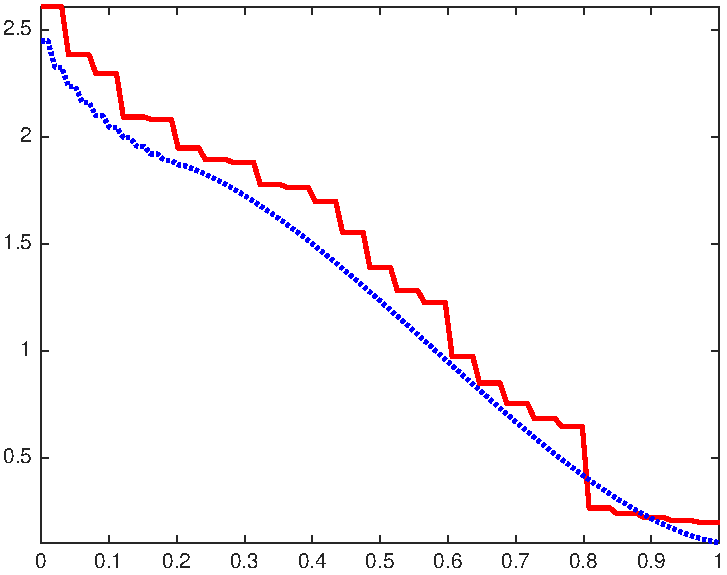
\includegraphics[width=0.75\columnwidth]{distrN100.pdf}\\$N=100$}%
\only<2>{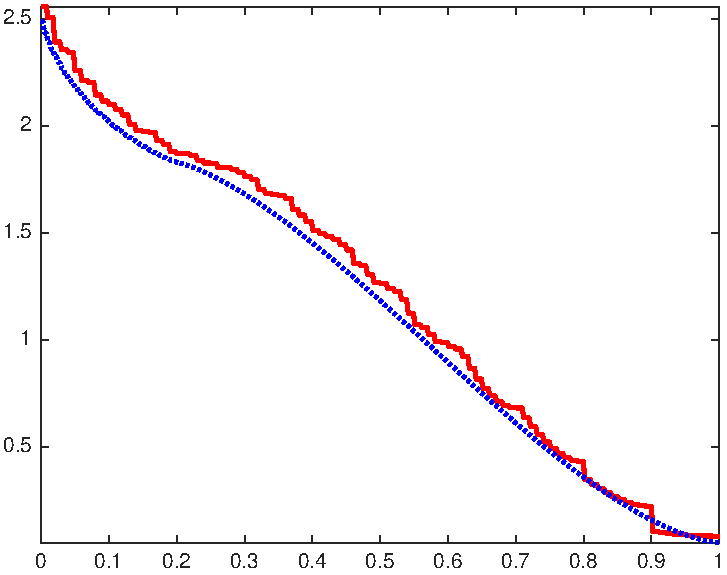
\includegraphics[width=0.75\columnwidth]{distrN400.pdf}\\$N=400$}%
\only<3>{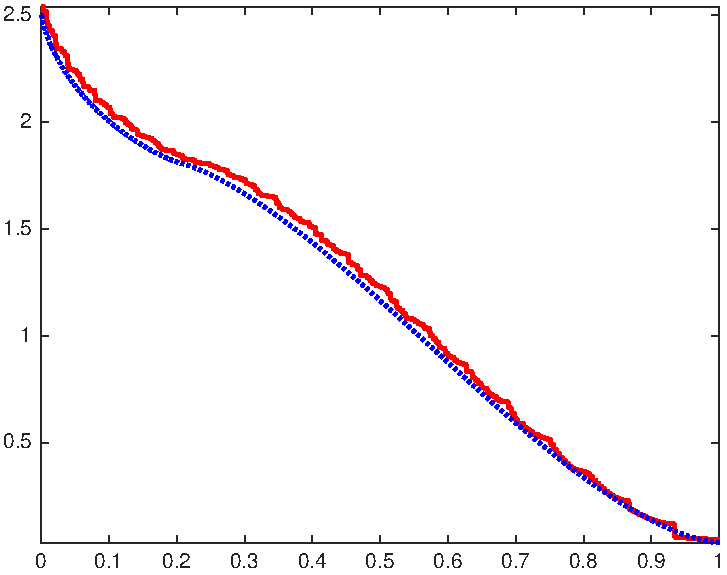
\includegraphics[width=0.75\columnwidth]{distrN900.pdf}\\$N=900$}%
\only<4>{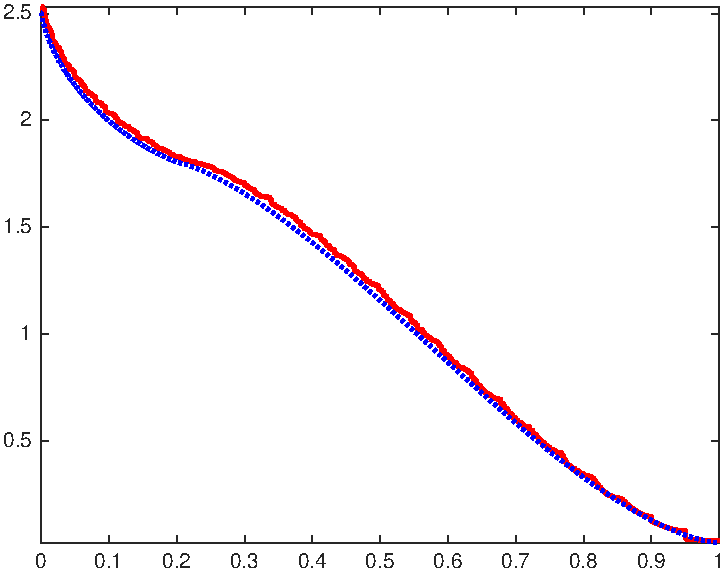
\includegraphics[width=0.75\columnwidth]{distrN1600.pdf}\\$N=1600$}%
\only<5>{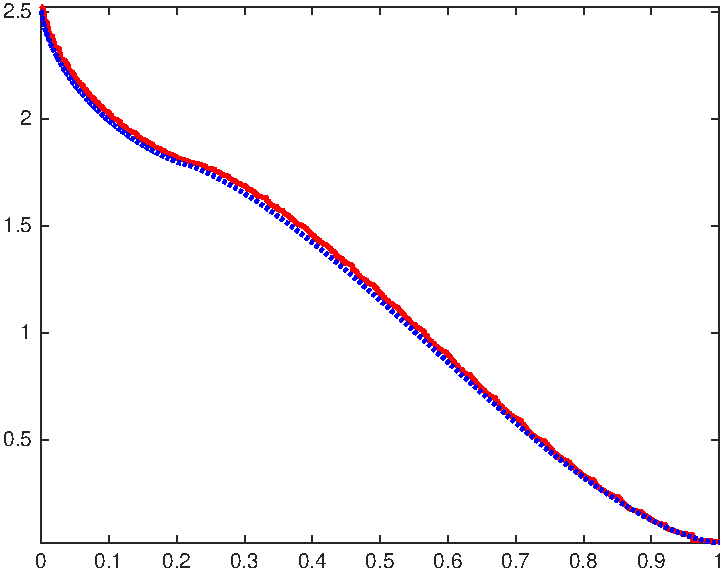
\includegraphics[width=0.75\columnwidth]{distrN2500.pdf}\\$N=2500$}%
\only<6>{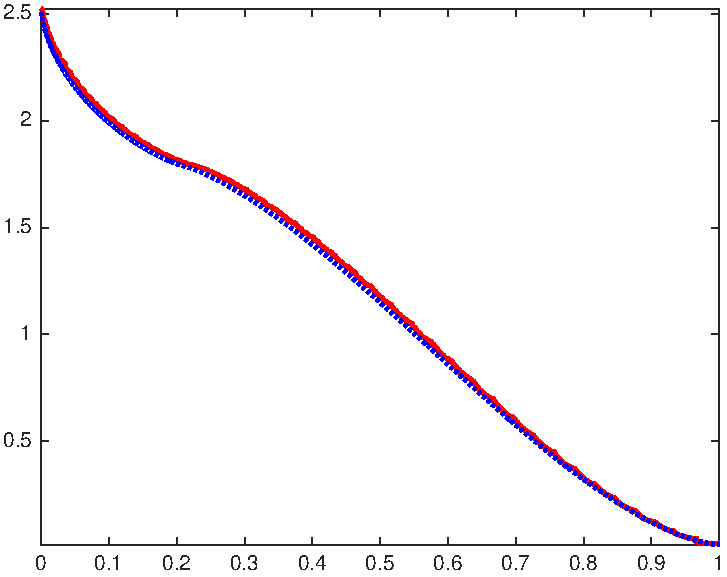
\includegraphics[width=0.75\columnwidth]{distrN3600.pdf}\\$N=3600$}%
\only<7>{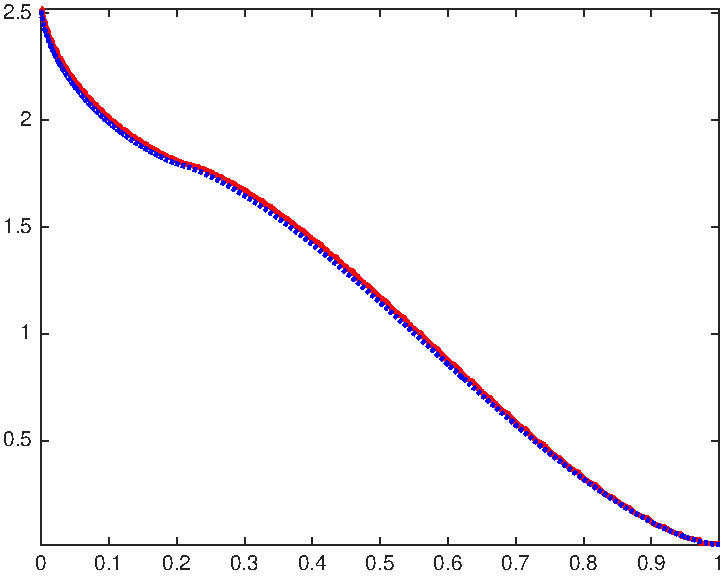
\includegraphics[width=0.75\columnwidth]{distrN4900.pdf}\\$N=4900$}%
\only<8>{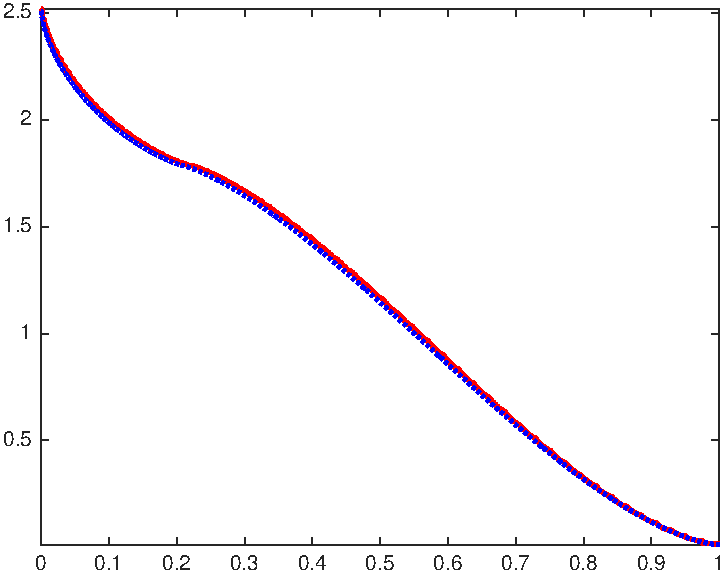
\includegraphics[width=0.75\columnwidth]{distrN6400.pdf}\\$N=6400$}%

\end{column}
\end{columns}

\end{frame}

\begin{frame}{GLT: a negative result for circulant matrices}
	
\faQuestionCircle\,And so we have the \textbf{asymptotic distribution} of our \textbf{singular values}, but what do we do with it?

\begin{itemize}
	\item[\alert{\faExclamationCircle}]<2-> The function
	\[
	k(x,\theta) = d^+(x)f_\alpha(\theta) + d^-(x) f_\alpha(-\theta) \text{ for } (x,\theta) \in [0,1] \times [-\pi,\pi],
	\]
	depends on \textbf{both} $x$ and $\theta$, on the other hand \textbf{any circulant preconditioner} will \textbf{depend only} on the \textbf{$\theta$ variable}!
	\item[$\Rightarrow$]<3-> \alert{No circulant preconditioner will ever cluster} the singular values of \alert{a sequence with a ``space variant'' spectral distribution}.
	\item[\faQuestionCircle]<4> What type of preconditioner can we use to solve this issue?
\end{itemize}

\end{frame}

\subsection{Structure preserving preconditioners}

\begin{frame}{\faLightbulb\,Structure preserving preconditioners}

The GLT class of sequences is a $*$-algebra, thus we can try to \textbf{proecondition} the sequence $\{A_N\}_N$ with \textbf{something from the same class}. We then look for:

\begin{itemize}
	\item[\faHammer]<2-> A sequence $\{P_N\}_N$ in the GLT class,
	\item[\faHammer]<3-> A sequence $\{P_N\}_N$ such that $\{ P_N^{-1} A_N\}_N \sim_{\rm GLT} 1$, 
	\item[\faHammer]<4-> A sequence $\{P_N\}_N$ that is \emph{easy enough} to invert.
\end{itemize}

\begin{exampleblock}<5->{\faBookReader\,An old idea anew}
This a modification of an old idea, if we take a Toeplitz system $T_n(f)$ then we can use $T_n(1/f)$ as a preconditioner!
\begin{itemize}
	\item[\faMagic] $P_n^{-1} = T_n(1/f)$ \textbf{is not the inverse} of $T_n(f)$,
	\item[\faMagic] \alert<6>{If we have} $T_n(1/f)$, its application cost is $O(n \log n)$,
	\item[\faExclamationCircle]<6-> Computing the Fourier coefficients of $1/f$ can be expensive.
\end{itemize}
\end{exampleblock}

\end{frame}

\begin{frame}{Preconditioning Toeplitz with Toeplitz}
	
We have expressed the Fourier coefficients of $f$ as
\[
t_k = \frac{1}{2\pi}\int_{0}^{2\pi} f(\theta) e^{-ik\theta}\,\mathrm{d}\theta, \qquad k=0,\pm1,\pm2,\ldots,
\]
we say that $f$ is 
\begin{itemize}
	\item[\faBook] of \textbf{analytic type} if $t_k = 0$ for $k < 0$, or
	\item[\faBook] of \textbf{coanalytic type} if $t_k = 0$ for $k > 0$.
\end{itemize}

\begin{alertblock}{Lemma}
Let $f$ be of analytic type (or respectively coanalytic type) and $a_0 \neq 0$. Then $T_n(f)$ is invertible if and only if $\nicefrac{1}{f}$ is bounded and of analytic type (or respectively coanalytic type). In either case, we have $T_n(1/f)T_n(f) = T_n(f) T_n(1/f) = I_n$, for $I_n$ is the identity matrix.
\end{alertblock}

	
\end{frame}

\begin{frame}{Preconditioning Toeplitz with Toeplitz}

\begin{alertblock}{Lemma \parencite{MR1230358}}
Let $f$ be a \textbf{positive} trigonometric polynomial of degree $K$ 
\[
f(\theta) = \sum_{k=-K}^{K} t_k e^{ik\theta}.
\]
Then for $n > 2K$, $\operatorname{rank}(T_n(1/f)T_n(f) - I_n) \leq 2K$.
\end{alertblock}

\textbf{Proof.} Let 
\[
\frac{1}{f(\theta)} = \sum_{k = -\infty}^{+\infty} \rho_k e^{ik\theta} \onslide<2->{\;\Rightarrow\; \sum_{k=-K}^{K} t_k \rho_{m-k} = \begin{cases}
1, & \text{ if } m = 0,\\
0, & \text{otherwise}.
\end{cases} }
\]
\onslide<3>{Thus for $n > 2K$, the entries of $T_n(1/f)T_n(f) - I_n$ are all zeros except possibly entries in its first and last $K$ columns. \hfill \qed}
\end{frame}

\begin{frame}[fragile]{Preconditioning Toeplitz with Toeplitz}
Given $|\alpha| < 1$ consider
\begin{columns}
\begin{column}{0.35\columnwidth}
\[
f(\theta) = \frac{1 + \alpha^2 - \alpha e^{i\theta} -\alpha e^{-i\theta}}{1-\alpha^2}
\]
$T_n(f)$ is tridiagonal and SPD.
\end{column}
\begin{column}{0.6\columnwidth}
\definecolor{bg}{rgb}{0.95,0.95,0.95}%
\begin{minted}[bgcolor=bg,fontsize=\small,breaklines]{matlab}
function T = kacmatrix(n,alpha)
%KACMATRIX Kac-Murdock-Szego matrices
e = ones(n,1);
T = spdiags(([-alpha,1+alpha^2,-alpha] ./(1-alpha^2)).*e,-1:1,n,n);
end
\end{minted}
\end{column}
\end{columns}
We can express
\[
\frac{1}{f(\theta)} = \sum_{k=-\infty}^{+\infty} t^{|k|} e^{ik\theta} = \frac{1-\alpha^2}{\left(1-\alpha e^{i\theta}\right) \left(1-\alpha e^{-i\theta}\right)},
\]
and $T_n(1/f)$ is then a \textbf{dense Toeplitz matrix}.
\end{frame}

\begin{frame}[fragile]{Preconditioning Toeplitz with Toeplitz}

We can compute the coefficients in an \textbf{inefficient way} and apply it to the CG/PCG
\begin{onlyenv}<1-3>
\begin{columns}
\begin{column}{0.25\columnwidth}
\centering
\only<1>{\begin{tabular}{ccc}
\toprule
$N$ & CG & PCG \\
\midrule
32 & 20 & 2 \\
64 & 20 & 2 \\
128 & 20 & 2 \\
256 & 20 & 2 \\
512 & 20 & 2 \\
1024 & 20 & 2 \\
2048 & 20 & 2 \\
\bottomrule
\end{tabular}

$\alpha = 0.5$}%
\only<2>{
\begin{tabular}{ccc}
	\toprule
	$N$ & CG & PCG \\
	\midrule
32 & 6 & 2 \\
64 & 6 & 2 \\
128 & 6 & 2 \\
256 & 6 & 2 \\
512 & 6 & 2 \\
1024 & 6 & 2 \\
2048 & 6 & 2 \\
	\bottomrule
\end{tabular}

$\alpha = 0.1$}%
\only<3>{
\begin{tabular}{ccc}
\toprule
$N$ & CG & PCG \\
\midrule
32 & 20 & 3 \\
64 & 20 & 2 \\
128 & 20 & 2 \\
256 & 20 & 2 \\
512 & 20 & 2 \\
1024 & 20 & 2 \\
2048 & 20 & 2 \\
\bottomrule
\end{tabular}

$\alpha = 0.8$}
\end{column}
\begin{column}{0.74\columnwidth}
\definecolor{bg}{rgb}{0.95,0.95,0.95}%
\begin{minted}[bgcolor=bg,fontsize=\small,breaklines]{matlab}
function T = invkacmatrix(n,alpha)
%INVKACMATRIX Gives back the 1/Kac-Murdock-Szego matrices
f = @(th) (1 - alpha^2)./((1-alpha*exp(1i*th)) .*(1-alpha*exp(-1i*th)));
c = zeros(n,1); r = zeros(1,n);
for k=1:n
 r(k) = integral(@(th) f(th).*exp(1i*th*(k-1)),0,2*pi) /(2*pi);
 c(k) = integral(@(th) f(th).*exp(-1i*th*(k-1)),0,2*pi) /(2*pi);
end
T = real(toeplitz(r,c));
end
\end{minted}
\end{column}
\end{columns}
\end{onlyenv}
\begin{onlyenv}<4>
	\[
	\operatorname{rank}\left( T_n(1/f)T_n(f) - I_n \right) = 2
	\]
\end{onlyenv}
\begin{onlyenv}<5>
\[
\operatorname{rank}\left( \vcenter{\hbox{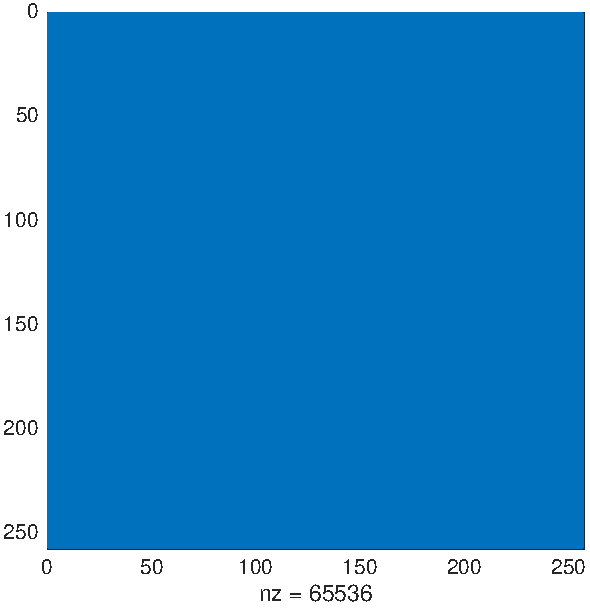
\includegraphics[width=0.2\columnwidth]{Tinv.pdf}}} \vcenter{\hbox{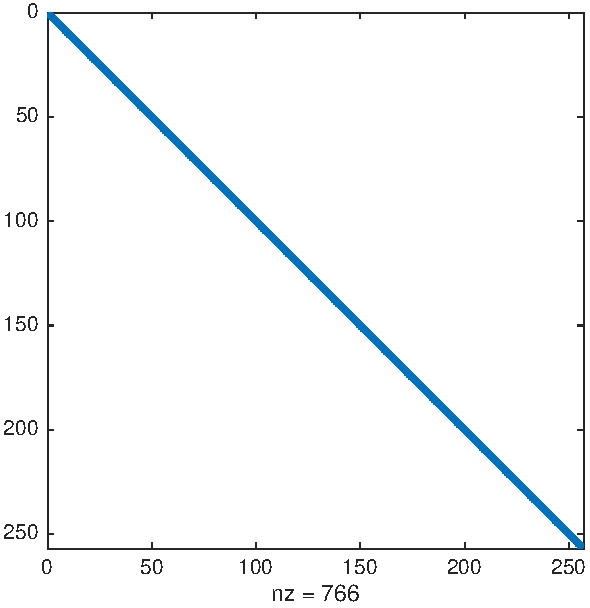
\includegraphics[width=0.2\columnwidth]{T.pdf}}} - \vcenter{\hbox{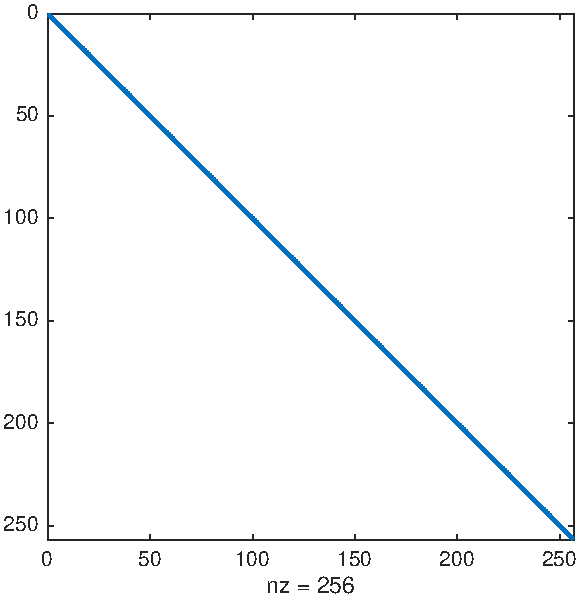
\includegraphics[width=0.2\columnwidth]{I.pdf}}} \right) = \vcenter{\hbox{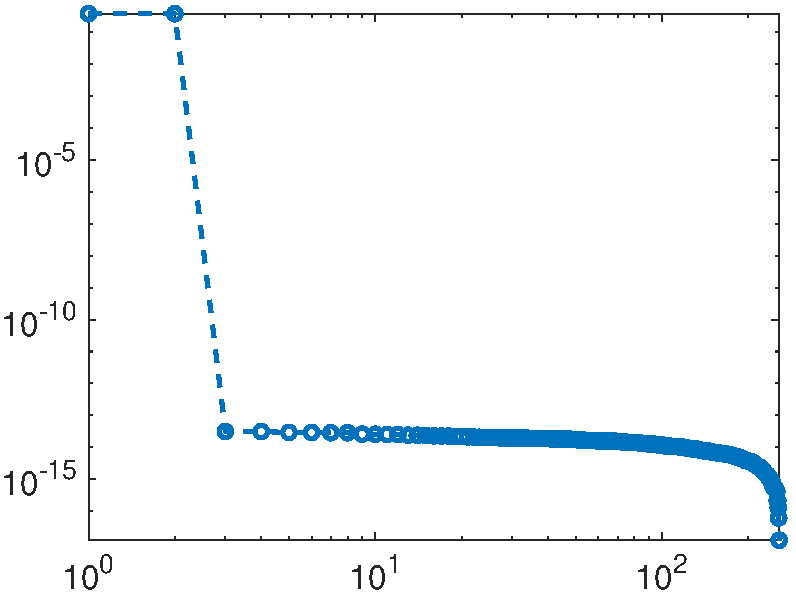
\includegraphics[width=0.25\columnwidth]{svd.pdf}}}
\]
\end{onlyenv}
\begin{onlyenv}<6->
	\[
	\operatorname{rank}\left( T_n(1/f)T_n(f) - I_n \right) = \vcenter{\hbox{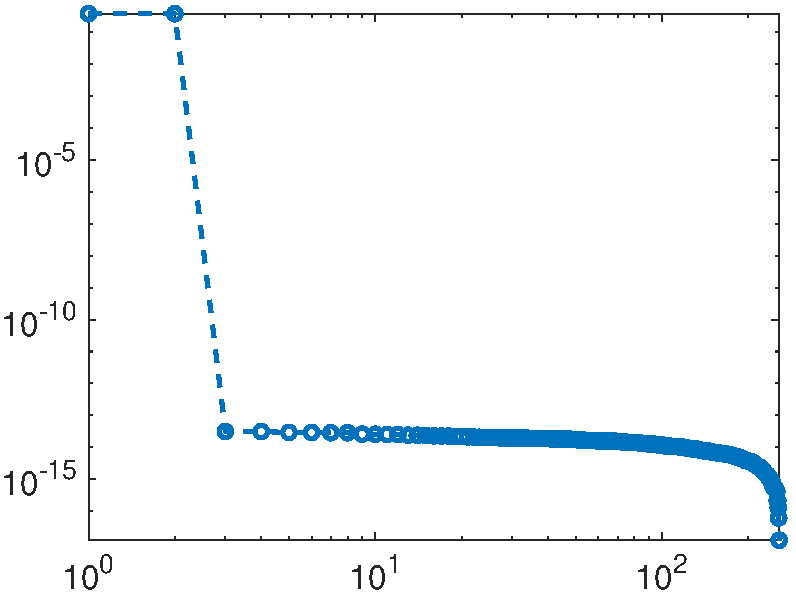
\includegraphics[width=0.4\columnwidth]{svd.pdf}}}
	\]
\begin{itemize}
	\item[\faPen] An \textbf{exercise} to make the evaluation and construction of the involved quantities would be using the \mintinline{matlab}{fft} to compute the Fourier coefficients of $1/f(\theta)$.
\end{itemize}
\end{onlyenv}

\end{frame}

\begin{frame}{Preconditioning Toeplitz with Toeplitz}

\begin{alertblock}{Lemma \parencite{MR1230358}}
Let $f$ be a positive $2\pi$-periodic continuous function. Then for all $\varepsilon > 0$, there exists positive integers $M$ and $N$ such that for all $n > N$,
\[
T_n(1/f) T_n(f) = I_n + L_n + U_n,
\text{where} \operatorname{rank}(L_n) \leq M  \text{ and }\|U_n\|_2 < \varepsilon.\]
\end{alertblock}

\textbf{Proof.} \only<1>{By the Weierstrass Theorem, there exists a positive trigonometric polynomial
\[
p_K(\theta) = \sum_{k = -K}^{+K} \rho_k e^{ik\theta}, \quad \rho_{-k} = \overline{\rho}_k, \text{ such that }
\nicefrac{\operatorname{f}_{\min}}{2} \leq p_K(\theta) \leq 2 f_{\max}\;\forall\,\theta \in [0,2\pi], \text{ and}
\]
\[
\max_{\theta \in [0,2\pi]} |f(\theta)-p_K(\theta)| \leq \frac{f_{\min}}{2}(-1 + \sqrt{1+\varepsilon}) \min \left\lbrace \frac{f_{\min}}{2 f_{\max}},1 \right\rbrace.
\]}\only<2-4>{
We write
\[
\begin{split}
T_n(1/f)T_n(f) = \only<2>{&\;T_n(1/f)T_n^{-1}(1/p_K) T_n(1/p_K)T_n(p_K) T_n^{-1}(p_K) T_n(f)\\
= &\;} (I_n + V_n) \left( T_n(1/p_K) T_n(p_K) \right) (I_n + W_n)
\end{split}
\]
\only<2>{where $V_n = ( T_n(1/f) - T_n(1/p_K)T_n^{-1}(1/p_K) )$ and $W_n = T_n^{-1}(p_k)(T_n(f) - T_n(p_K))$}
\only<3-4>{and by the property of the generating functions and the Weierstrass Theorem
\[
\begin{split}
\|T_n^{-1}(p_K)\|_2 \leq \frac{2}{f_{\min}}, \; \|T_n^{-1}(1/p_K)\|_2 \leq 2 f_{\max}, \; \|T_n(f) - T_n(p_K)\|_2 \leq \frac{(-1 + \sqrt{1+\varepsilon}) f_{\min}}{2}, \\
\| T_n(1/f) - T_n(1/p_K)\|_2 \only<3>{\leq \max_{\theta in [0,2\pi]} \left\lvert \frac{1}{f(\theta)} - \frac{1}{p_K(\theta)}\right\rvert} \leq \frac{2}{f_{\min}^2} \max_{\theta \in [0,2\pi]} |f(\theta) - p_K(\theta)| \only<4>{ \leq \frac{-1 + \sqrt{1+\varepsilon}}{2 f_{\max}}. }
\end{split} 
\]
}
}%
\only<5->{
We write
\[
T_n(1/f)T_n(f) = (I_n + V_n) \only<5>{\left( T_n(1/p_K) T_n(p_K) \right)}\only<6->{ ( I_n + \tilde{L}_n ) } (I_n + W_n)\only<5-6>{.} \only<7>{\equiv I_n + L_n + U_n,}
\]
\only<5-6>{Using the \textbf{lemma on trigonometric polynomials} and using $n > 2K$ we have
\[
T_n(1/p_K)T_n(p_K) = I_n + \tilde{L}_n \text{ with } \operatorname{rank}(\tilde{L}_n) \leq 2K.
\]}%
\only<7>{where
\[
U_n = V_n + W_n + V_n W_n, \quad L_n = \tilde{L}_n(I_n + W_n) + V_n \tilde{L}_n(I_n + W_n),
\]
and using the previous relations
\[
\operatorname{rank}(L_n) \leq 4K, \text{ and } \|U_n\|_2 \leq \varepsilon. \hfill\qed
\]
}
}


\end{frame}

\begin{frame}{Preconditioning Toeplitz with Toeplitz}

\begin{alertblock}{Theorem \parencite{MR1230358}}
Let $f$ be a \textbf{positive} $2\pi$-periodic continuous function. Then for all $\varepsilon > 0$, there exist positive integers $M$ and $N$ such that for all $n > N$, at most $M$ eigenvalues of $T_n(1/f)T_n(f) - I_n$ have absolute value greater than $\varepsilon$.
\end{alertblock}

\textbf{Proof (idea).} The HPD matrix $X_n = T_n^{\nicefrac{1}{2}}(1/f) T_n(f) T_n^{\nicefrac{1}{2}}(1/f) \sim T_n(1/f)T_n(f)$. Use the decomposition of the previous Theorem and the uniform boundedness of~$T_n^{\pm\nicefrac{1}{2}}(1/f)$. \qed

\begin{itemize}
	\item[\faBomb]<2-> We still need \textbf{positive} generating functions,
	\item[\faCogs]<3-> If $f$ is not given explicitly or the evaluation of $1/f(\theta)$ are costly the approach is infeasible.
	\item[{\faLightbulb[regular]}]<4-> The \textbf{idea} from \parencite{MR1230358} is to reduce the cost of working with $f$ and $1/f$ by using convolution products with Kernel functions.
\end{itemize}

\end{frame}

\begin{frame}{Preconditioning GLT with GLT}
	
GLT sequences are a $*$-algebra, some of the analysis is therefore greatly simplified.
\begin{alertblock}{Theorem \parencite[Section 8.4]{MR3674485} }
	Let $\{A_N\}_N$ be a \alert<3>{sequence of Hermitian matrices} such that $\{A_N\}_N\sim_{ GLT}\kappa$, and let $\{P_N\}_N$ be a \alert<3>{sequence of Hermitian positive definite matrices} such that $\{P_N\}_N\sim_{GLT}\xi$ and \alert<2>{$\xi\ne0$ a.e.} Then 
	\[ \{P_N^{-1}A_N\}_N\sim_{\rm GLT}\xi^{-1}\kappa,\qquad \{P_N^{-1}A_N\}_N\sim_{\sigma,\,\lambda}(\xi^{-1}\kappa,\mathcal{I}^d). \]
\end{alertblock}
	
\begin{itemize}
	\item[{\definecolor{success}{HTML}{4a934a}\textcolor{success}{\faSmile}}]<2-> We need less than positive!
	\item[\faWrench]<3-> If we move to the non-symmetric case, we are left just with a relation with respect to the singular values.
	\item[\faMagic]<4-> The \alert{\textbf{general idea for a GLT preconditioner}} is then to find a GLT sequence $\{P_N\}_N$
	\begin{itemize}
		\item \normalsize that is easy to invert,
		\item \normalsize and such that $\xi^{1} \kappa = 1$ or \emph{at least} a quantity bounded and bounded away from zero.
	\end{itemize}
\end{itemize}
	
\end{frame}

\begin{frame}{Preconditioning GLT with GLT}
	
Let us finally go back to our case of interest
\[
A_N = \nu I_N - \left( D_N^+ G_N + D_N^- G_N^T \right),
\]
we build a preconditioner with the \textbf{same structure} such that
\begin{itemize}
	\item[\faCogs] we have a \emph{small bandwidth} $\Rightarrow$ a \textbf{small computational cost},
	\item[\alert{\faBomb}]<2-> the symbol of a bandwidth Toeplitz
	matrix is a trigonometric polynomial, hence the \textbf{zero of the symbol cannot be of fractional order}.
	\item[\faLightbulb]<3-> $P_{1,N} = \nu I + D^+_N B_N + D^-_N B_N^T$, $B_n = T_n(1 - exp(-i\theta))$,
	\item[\faBook]<5-> $\{P_{1,N}\}_N \sim_{GLT} p_1(x,\theta) = d_+(x)(1-e^{-i\theta}) + d_-(x)(1-e^{i\theta})$, holds only in the singular value sense!
	\item[\faLightbulb]<4-> $P_{2,N} = \nu I + D^+_N L_N + D^-_N L_N^T$, $B_n = T_n(2 - 2\cos(\theta))$
	\item[\faBook]<6-> $\{P_{2,N}\}_N \sim_{GLT} p_2(x,\theta) = (d_+(x) + d_-(x))(2-2\cos(\theta))$, holds also in the eigenvalue sense!
\end{itemize}
\end{frame}

\begin{frame}{Preconditioning GLT with GLT}
	\alert{\faBomb} Since the symbol of a bandwidth Toeplitz
	matrix is a trigonometric polynomial, hence the \textbf{zero of the symbol cannot be of fractional order}:
	\[
	d_{\pm}(x,t) = d > 0\,:\;\lim_{\theta \rightarrow 0} \frac{h(x,\theta)}{p_k(x,\theta)} = +\infty, \qquad k \in \{1,2\}.
	\]
	
\begin{alertblock}<2->{Theorem \parencite[Theorem 3.1]{MR1480523}}
Let $f$ be an integrable function defined on $[-\pi,\pi]$ having in $x = x_0$ the unique zero of order $\rho$. Then, by choosing $2k$ the even number which minimizes the distance from $\rho$ and setting $g = |x-x_0|^{2k}$, the condition number of $T_n(g)^{-1} T_n(f)$ is asymptotical to $n^{2k-\rho}$.
\end{alertblock}

\begin{exampleblock}<3->{In our case}
We expect the condition number of the preconditioned matrix to be $O(N^{|\alpha-k|})$, $k \in \{1,2\}$.
\end{exampleblock}

\end{frame}

\begin{frame}{Preconditioning GLT with GLT}
Let's numerically test our idea.
\begin{columns}
\begin{column}{0.5\columnwidth}\centering
\only<1>{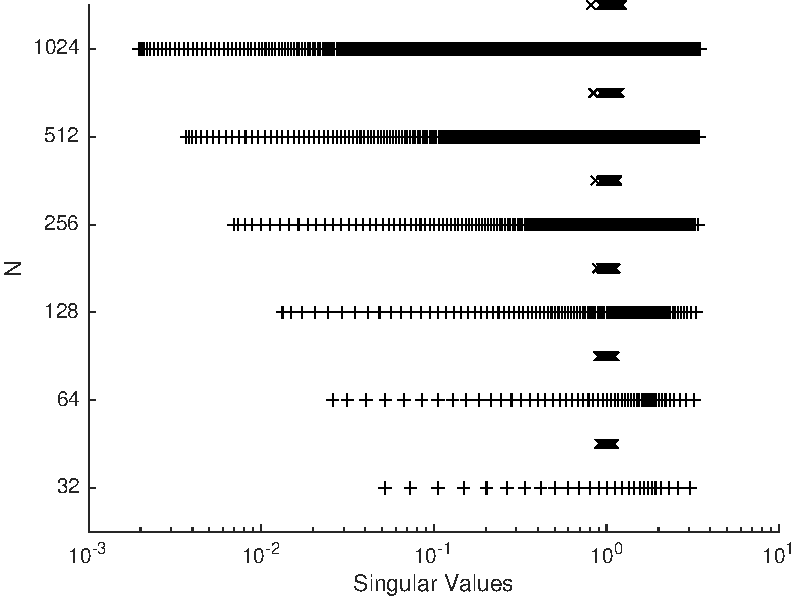
\includegraphics[width=\columnwidth]{spec_19_k2.pdf}\\$\alpha=1.9$, $k=2$}%
\only<2>{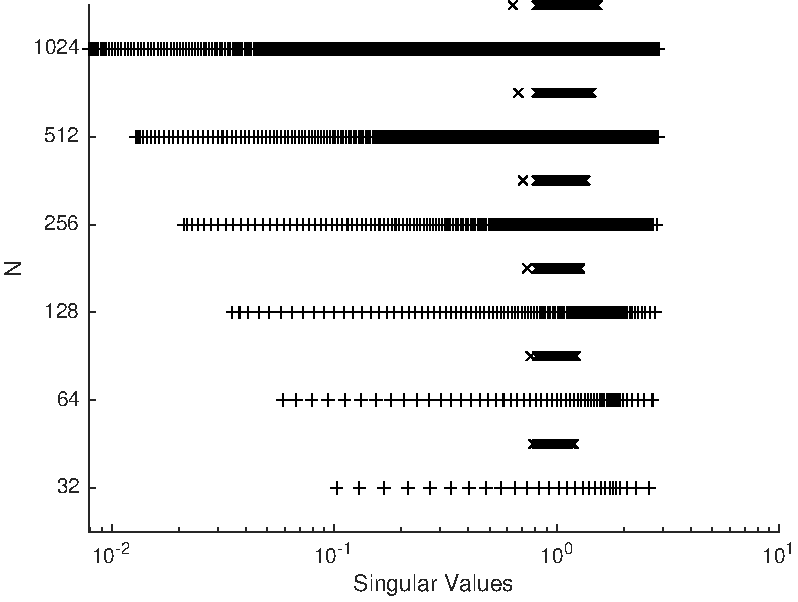
\includegraphics[width=\columnwidth]{spec_17_k2.pdf}\\$\alpha=1.7$, $k=2$}%
\only<3>{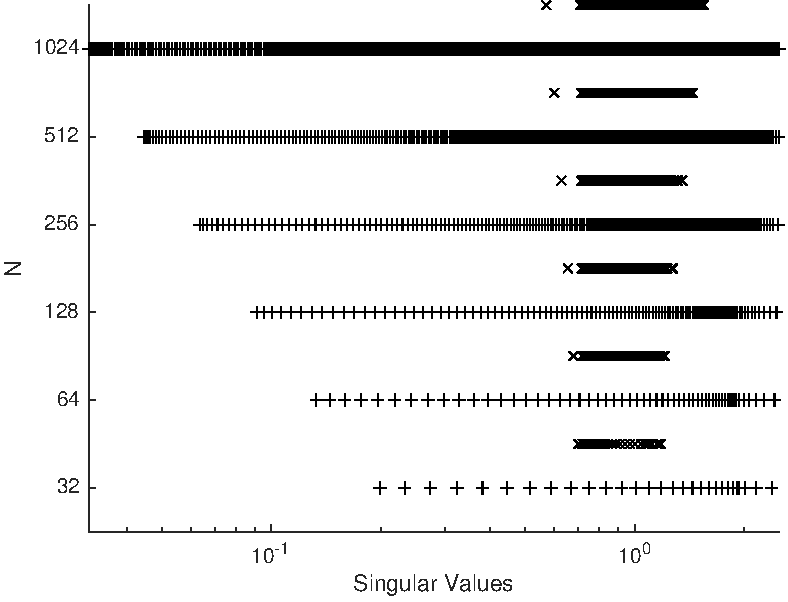
\includegraphics[width=\columnwidth]{spec_15_k2.pdf}\\$\alpha=1.5$, $k=2$}%
\only<4>{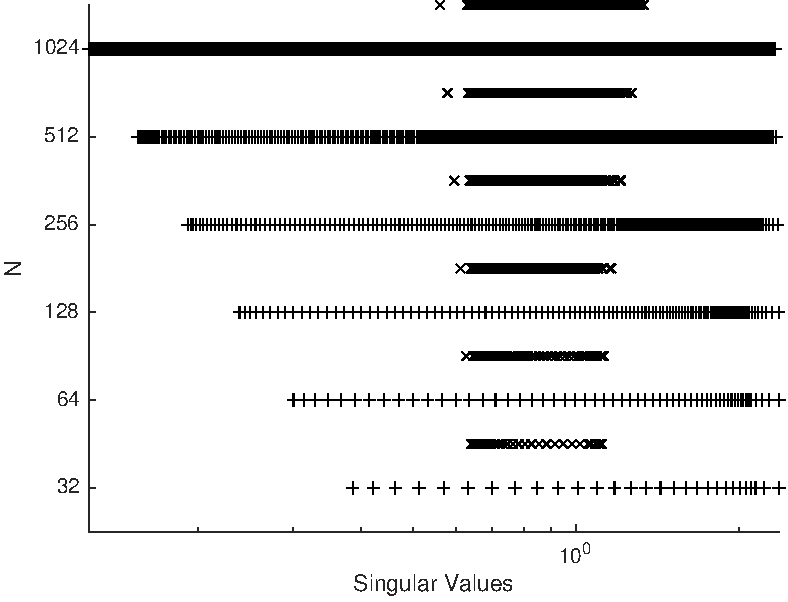
\includegraphics[width=\columnwidth]{spec_13_k2.pdf}\\$\alpha=1.3$, $k=2$}%
\only<5>{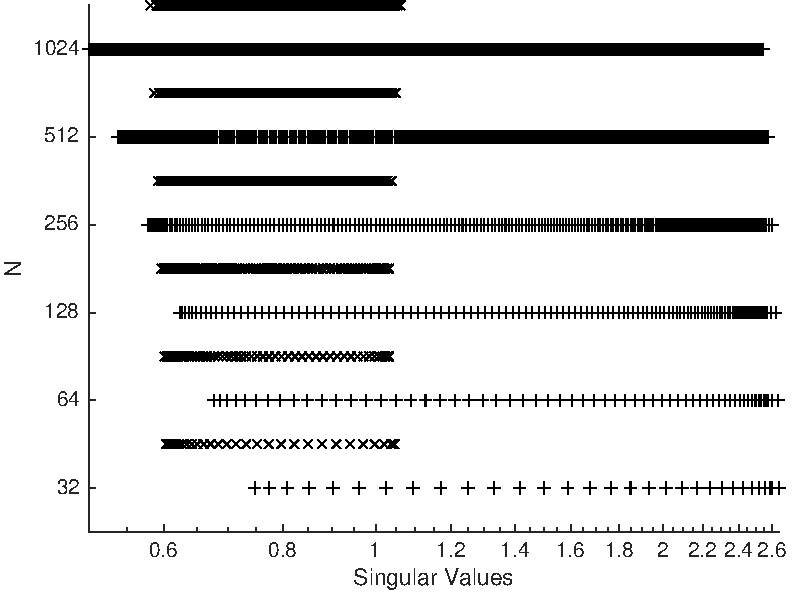
\includegraphics[width=\columnwidth]{spec_11_k2.pdf}\\$\alpha=1.1$, $k=2$}%
\only<6>{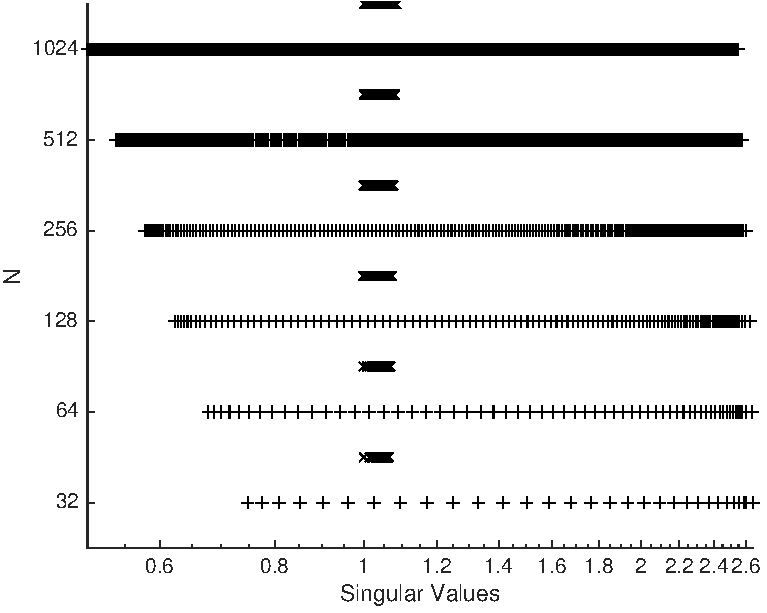
\includegraphics[width=\columnwidth]{spec_11_k1.pdf}\\$\alpha=1.1$, $k=1$}%
\only<7>{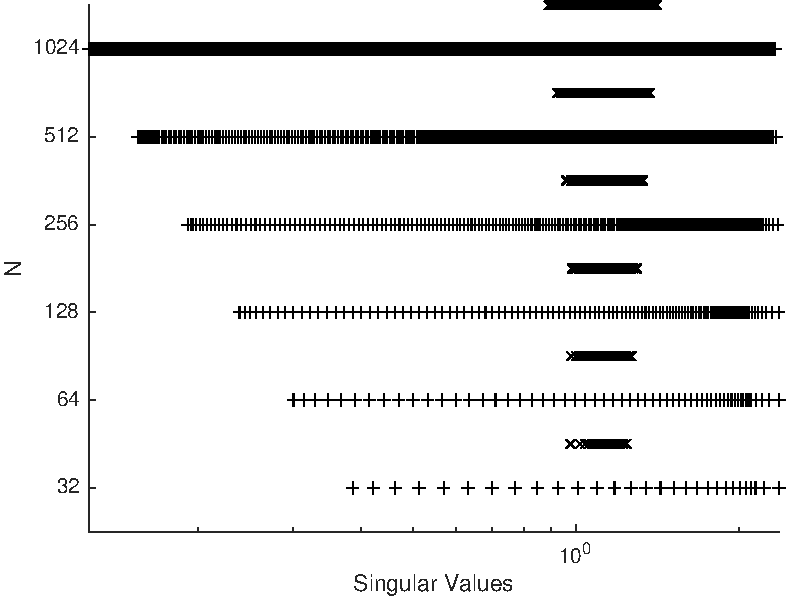
\includegraphics[width=\columnwidth]{spec_13_k1.pdf}\\$\alpha=1.3$, $k=1$}%
\only<8>{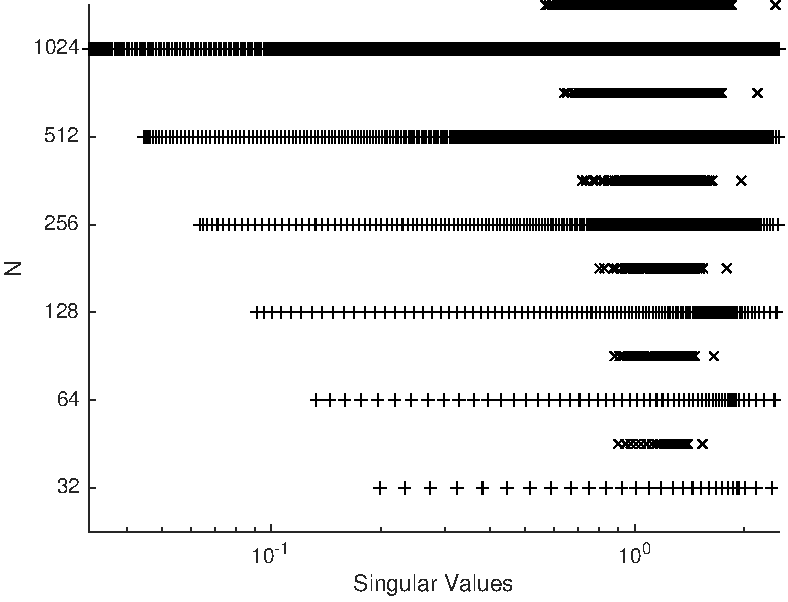
\includegraphics[width=\columnwidth]{spec_15_k1.pdf}\\$\alpha=1.5$, $k=1$}%
\only<9>{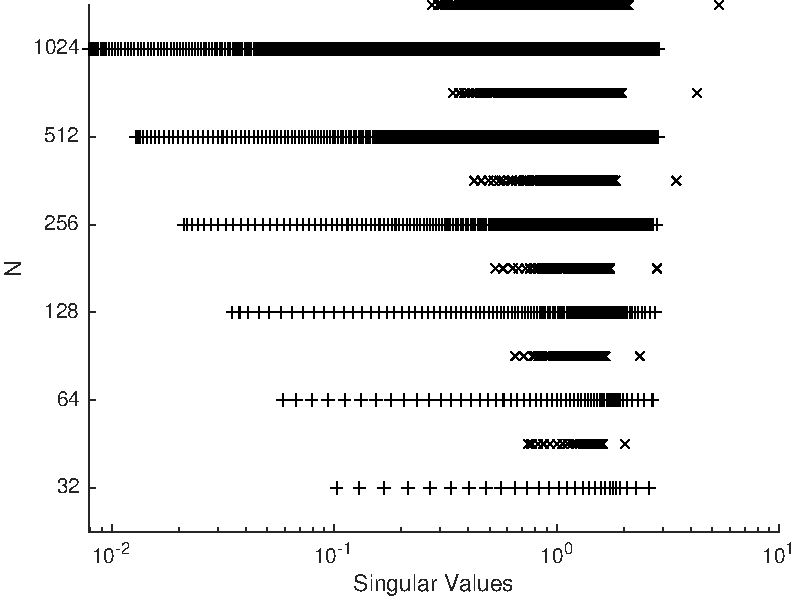
\includegraphics[width=\columnwidth]{spec_17_k1.pdf}\\$\alpha=1.7$, $k=1$}%
\only<10>{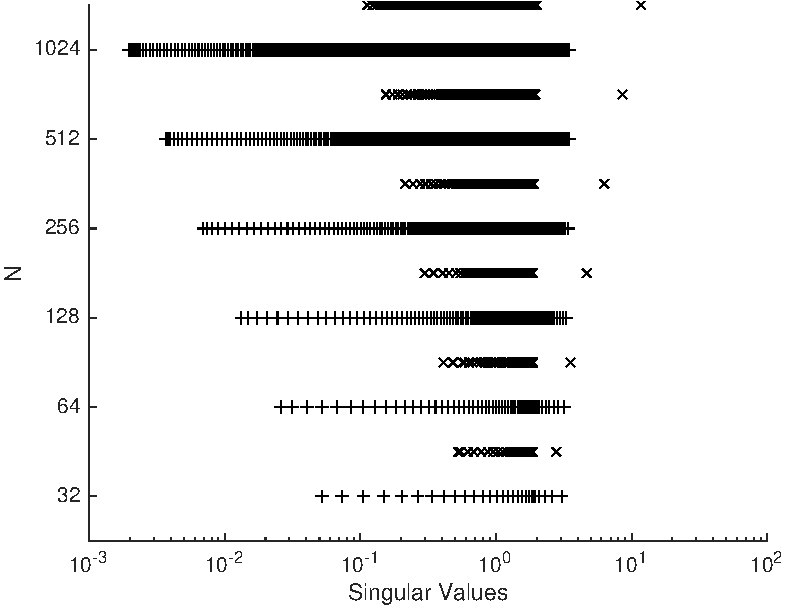
\includegraphics[width=\columnwidth]{spec_19_k1.pdf}\\$\alpha=1.3$, $k=1$}%
\end{column}
\begin{column}{0.5\columnwidth}\centering
\only<1>{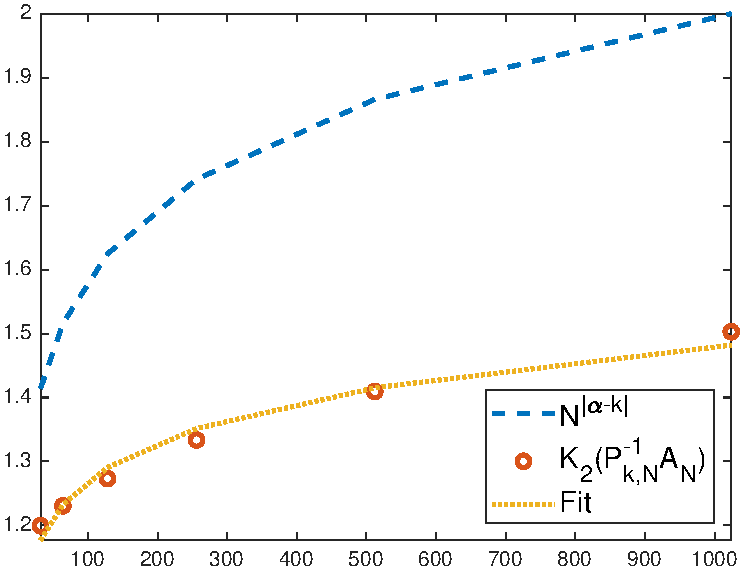
\includegraphics[width=\columnwidth]{cond_19_k2.pdf}}%
\only<2>{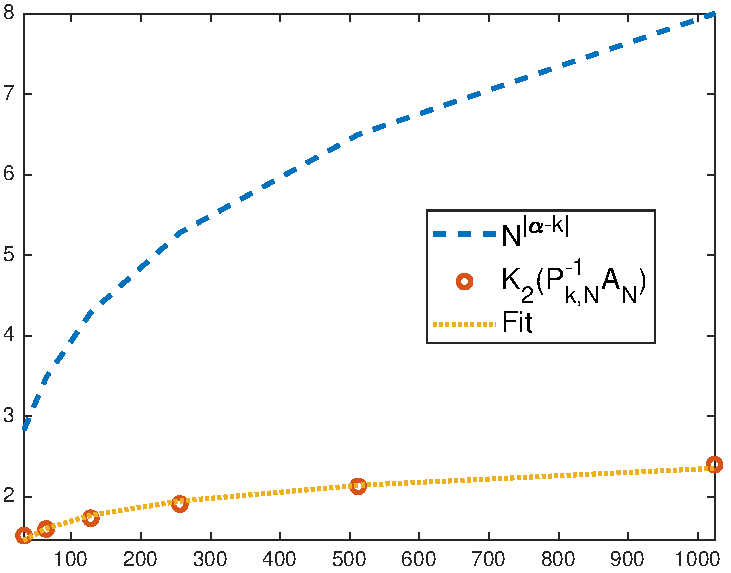
\includegraphics[width=\columnwidth]{cond_17_k2.pdf}\\$\alpha=1.7$, $k=2$}%
\only<3>{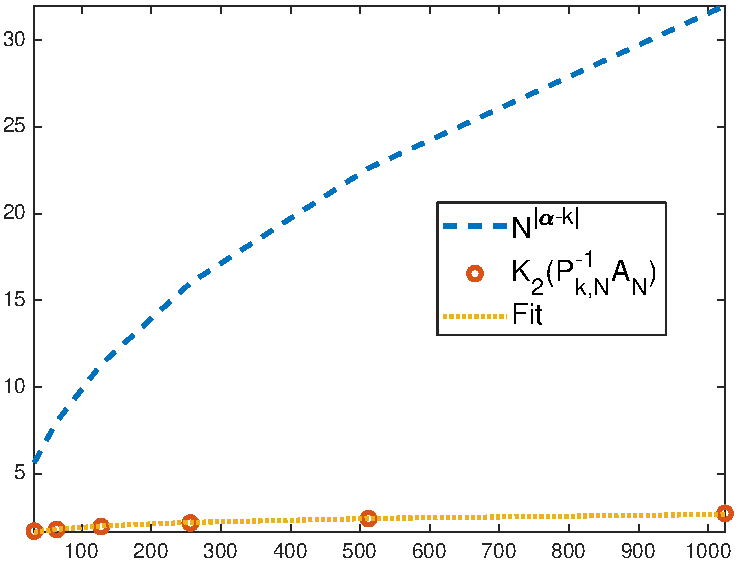
\includegraphics[width=\columnwidth]{cond_15_k2.pdf}\\$\alpha=1.5$, $k=2$}%
\only<4>{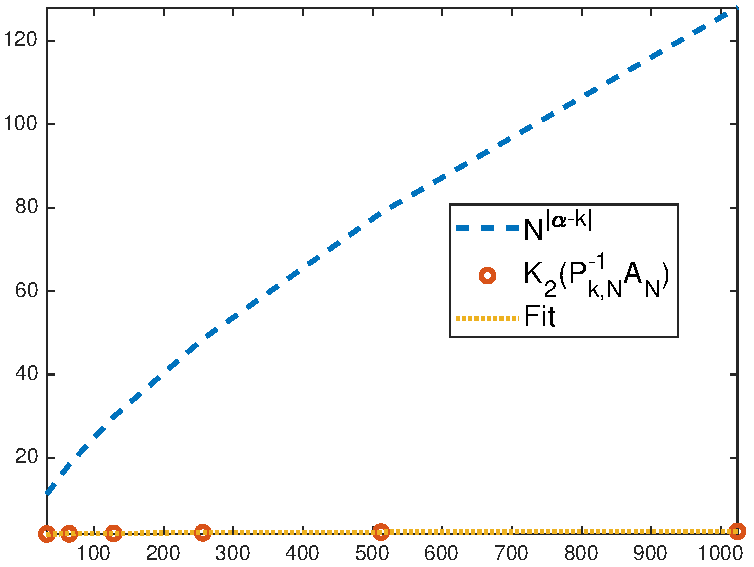
\includegraphics[width=\columnwidth]{cond_13_k2.pdf}\\$\alpha=1.3$, $k=2$}%
\only<5>{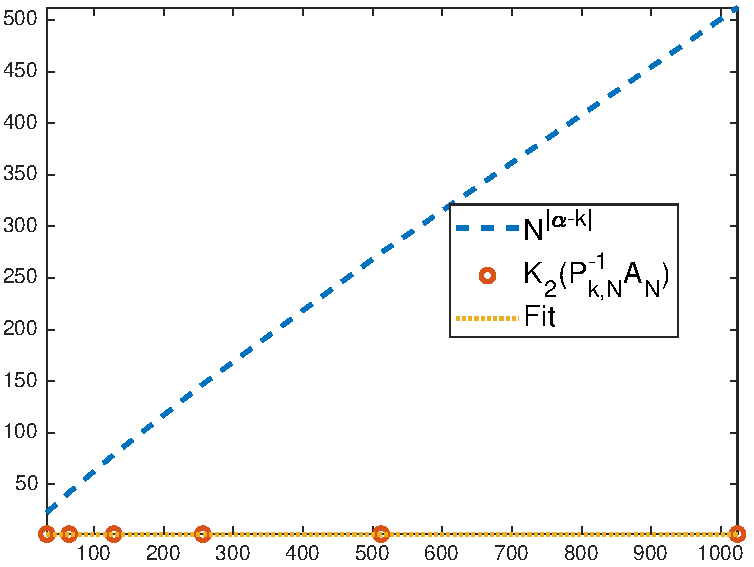
\includegraphics[width=\columnwidth]{cond_11_k2.pdf}\\$\alpha=1.1$, $k=2$}%
\only<6>{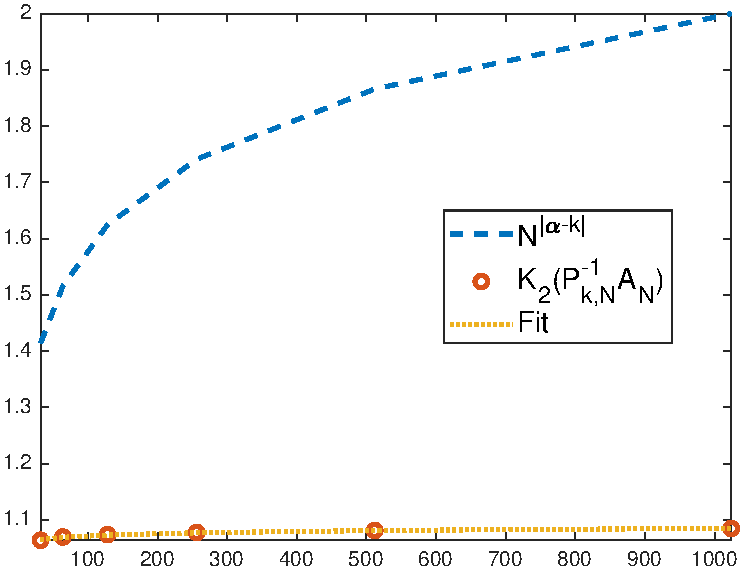
\includegraphics[width=\columnwidth]{cond_11_k1.pdf}\\$\alpha=1.1$, $k=1$}%
\only<7>{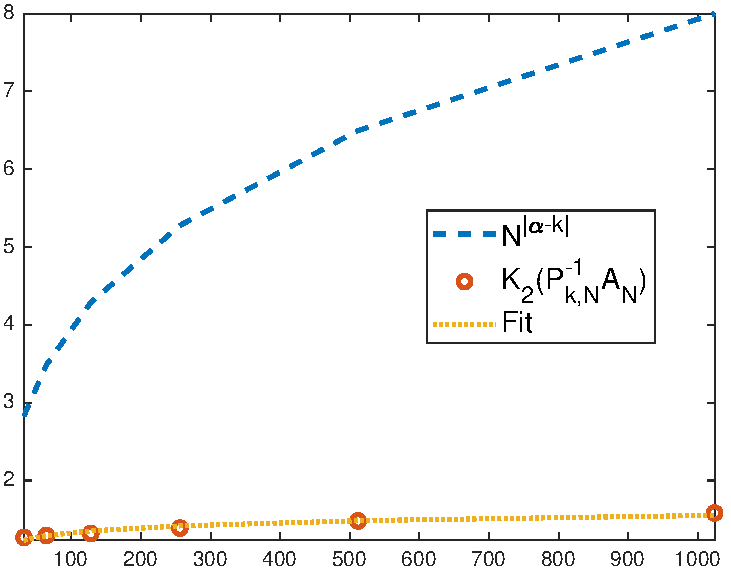
\includegraphics[width=\columnwidth]{cond_13_k1.pdf}\\$\alpha=1.3$, $k=1$}%
\only<8>{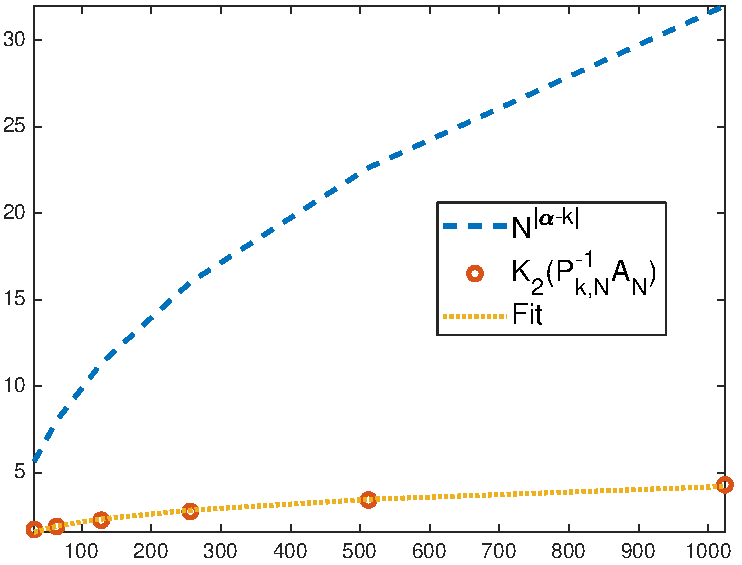
\includegraphics[width=\columnwidth]{cond_15_k1.pdf}\\$\alpha=1.5$, $k=1$}%
\only<9>{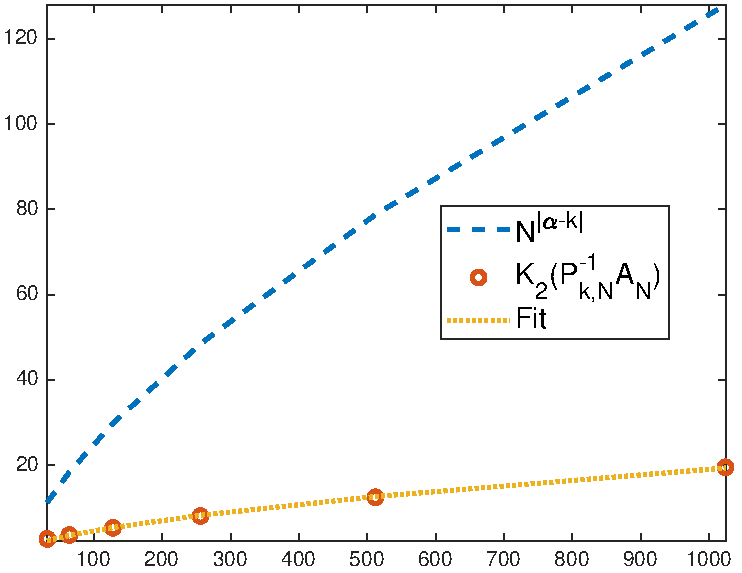
\includegraphics[width=\columnwidth]{cond_17_k1.pdf}\\$\alpha=1.7$, $k=1$}%
\only<10>{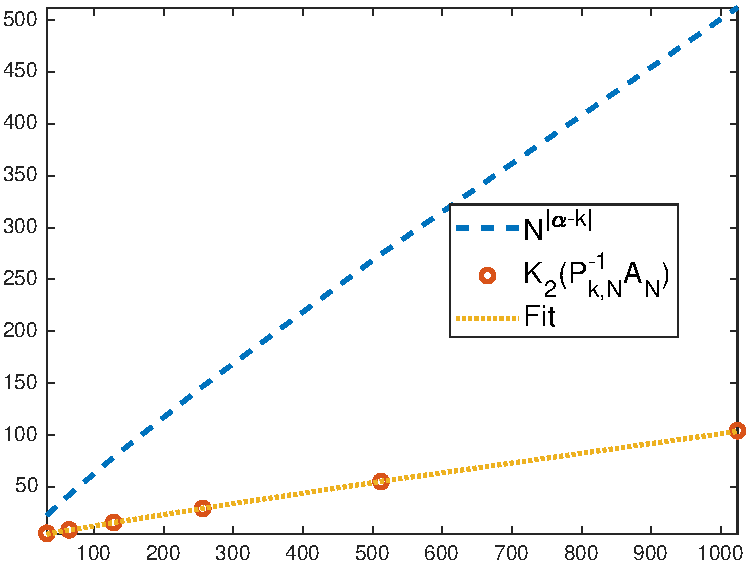
\includegraphics[width=\columnwidth]{cond_19_k1.pdf}\\$\alpha=1.3$, $k=1$}%
\end{column}
\end{columns}
\end{frame}

\begin{frame}{Preconditioning GLT with GLT}
Test case is
\[
d^+(x,t) = \Gamma(3-\alpha)x^\alpha, \qquad d^-(x,t) = \Gamma(3-\alpha) (2-x)^\alpha 
\]\vspace{-0.5em}
\begin{columns}
\begin{column}{0.5\columnwidth}\centering
\begin{onlyenv}<1>
\begin{tabular}{llllll}
	\toprule
	$\alpha$ & $N$ & GMRES & P & $P_{1,N}$ & $P_{2,N}$ \\
	\midrule
	1.2 & $2^{5}$ & 31 & 13 & 10 & 13\\
	& $2^{6}$ & 50 & 14 & 11 & 15 \\
	& $2^{7}$ & 64 & 14 & 11 & 16 \\
	& $2^{8}$ & 75 & 15 & 11 & 16 \\
	& $2^{9}$ & 84 & 15 & 11 & 16 \\
	& $2^{10}$ & 91 & 14 & 10 & 16 \\
	& $2^{11}$ & 96 & 14 & 10 & 16 \\
	\bottomrule
\end{tabular}
\end{onlyenv}
\begin{onlyenv}<2>
	\begin{tabular}{llllll}
		\toprule
		$\alpha$ & $N$ & GMRES & P & $P_{1,N}$ & $P_{2,N}$ \\
		\midrule
 1.3 & $2^{5}$ & 31 & 13 & 13 & 14\\
& $2^{6}$ & 55 & 14 & 15 & 15 \\
& $2^{7}$ & 79 & 15 & 16 & 16 \\
& $2^{8}$ & 100 & 15 & 16 & 17 \\
& $2^{9}$ & 119 & 15 & 16 & 17 \\
& $2^{10}$ & 136 & 15 & 17 & 17 \\
& $2^{11}$ & 153 & 15 & 17 & 17 \\
		\bottomrule
	\end{tabular}
\end{onlyenv}
\begin{onlyenv}<3>
	\begin{tabular}{llllll}
		\toprule
		$\alpha$ & $N$ & GMRES & P & $P_{1,N}$ & $P_{2,N}$ \\
		\midrule
 1.4 & $2^{5}$ & 31 & 13 & 16 & 13\\
& $2^{6}$ & 59 & 14 & 20 & 15 \\
& $2^{7}$ & 92 & 15 & 23 & 16 \\
& $2^{8}$ & 127 & 15 & 25 & 16 \\
& $2^{9}$ & 161 & 15 & 26 & 17 \\
& $2^{10}$ & 196 & 15 & 28 & 17 \\
& $2^{11}$ & 231 & 15 & 29 & 17 \\
		\bottomrule
	\end{tabular}
\end{onlyenv}
\begin{onlyenv}<4>
	\begin{tabular}{llllll}
		\toprule
		$\alpha$ & $N$ & GMRES & P & $P_{1,N}$ & $P_{2,N}$ \\
		\midrule
 1.5 & $2^{5}$ & 32 & 13 & 19 & 12\\
& $2^{6}$ & 61 & 14 & 25 & 14 \\
& $2^{7}$ & 104 & 15 & 32 & 15 \\
& $2^{8}$ & 155 & 15 & 38 & 15 \\
& $2^{9}$ & 209 & 15 & 43 & 16 \\
& $2^{10}$ & 268 & 15 & 49 & 16 \\
& $2^{11}$ & 332 & 15 & 54 & 16 \\
		\bottomrule
	\end{tabular}
\end{onlyenv}
\begin{onlyenv}<5>
	\begin{tabular}{llllll}
		\toprule
		$\alpha$ & $N$ & GMRES & P & $P_{1,N}$ & $P_{2,N}$ \\
		\midrule
 1.6 & $2^{5}$ & 32 & 13 & 22 & 11\\
& $2^{6}$ & 62 & 13 & 31 & 12 \\
& $2^{7}$ & 112 & 14 & 42 & 13 \\
& $2^{8}$ & 183 & 14 & 55 & 14 \\
& $2^{9}$ & 262 & 14 & 69 & 14 \\
& $2^{10}$ & 353 & 14 & 84 & 15 \\
& $2^{11}$ & 456 & 14 & 101 & 15 \\
		\bottomrule
	\end{tabular}
\end{onlyenv}
\begin{onlyenv}<6>
	\begin{tabular}{llllll}
		\toprule
		$\alpha$ & $N$ & GMRES & P & $P_{1,N}$ & $P_{2,N}$ \\
		\midrule
 1.7 & $2^{5}$ & 32 & 12 & 25 & 10\\
& $2^{6}$ & 64 & 13 & 38 & 11 \\
& $2^{7}$ & 118 & 13 & 55 & 12 \\
& $2^{8}$ & 207 & 13 & 77 & 12 \\
& $2^{9}$ & 319 & 13 & 104 & 12 \\
& $2^{10}$ & 449 & 13 & 136 & 13 \\
& $2^{11}$ & 605 & 13 & 176 & 13 \\
		\bottomrule
	\end{tabular}
\end{onlyenv}
\begin{onlyenv}<7->
	\begin{tabular}{llllll}
		\toprule
		$\alpha$ & $N$ & GMRES & P & $P_{1,N}$ & $P_{2,N}$ \\
		\midrule
 1.8 & $2^{5}$ & 32 & 12 & 27 & 9\\
& $2^{6}$ & 64 & 12 & 44 & 9 \\
& $2^{7}$ & 126 & 13 & 71 & 10 \\
& $2^{8}$ & 225 & 13 & 108 & 10 \\
& $2^{9}$ & 378 & 13 & 157 & 10 \\
& $2^{10}$ & 559 & 12 & 219 & 10 \\
& $2^{11}$ & 779 & 12 & 298 & 10 \\
		\bottomrule
	\end{tabular}
\end{onlyenv}
\end{column}
\begin{column}{0.5\columnwidth}
\only<1>{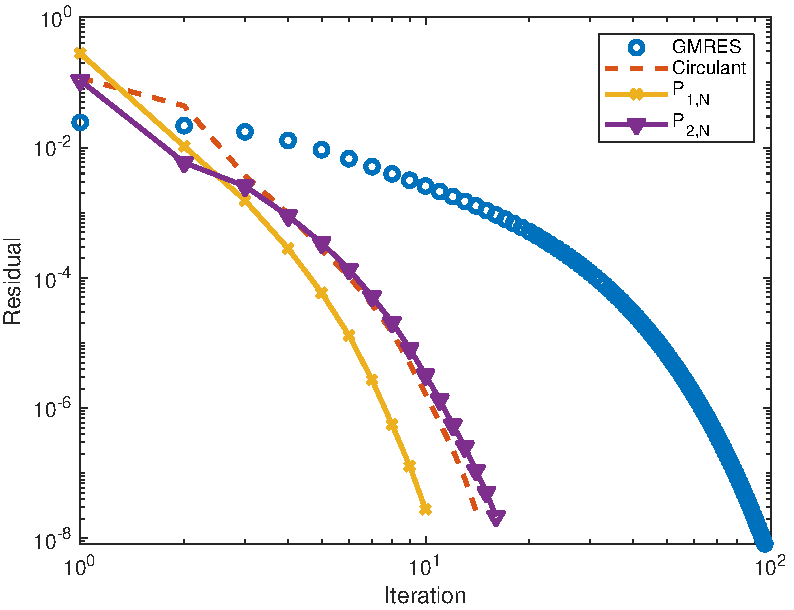
\includegraphics[width=\columnwidth]{gmresN=2048alpha=1.2_glt.pdf}}%
\only<2>{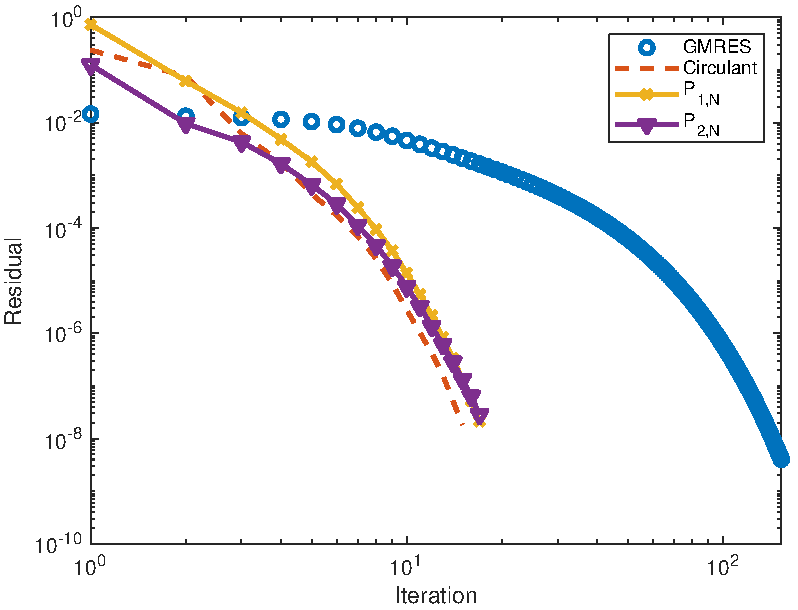
\includegraphics[width=\columnwidth]{gmresN=2048alpha=1.3_glt.pdf}}%
\only<3>{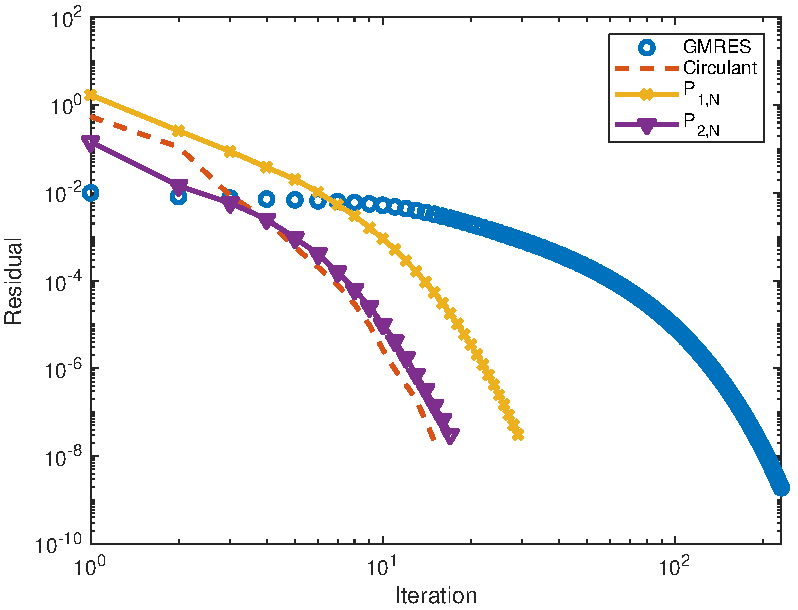
\includegraphics[width=\columnwidth]{gmresN=2048alpha=1.4_glt.pdf}}%
\only<4>{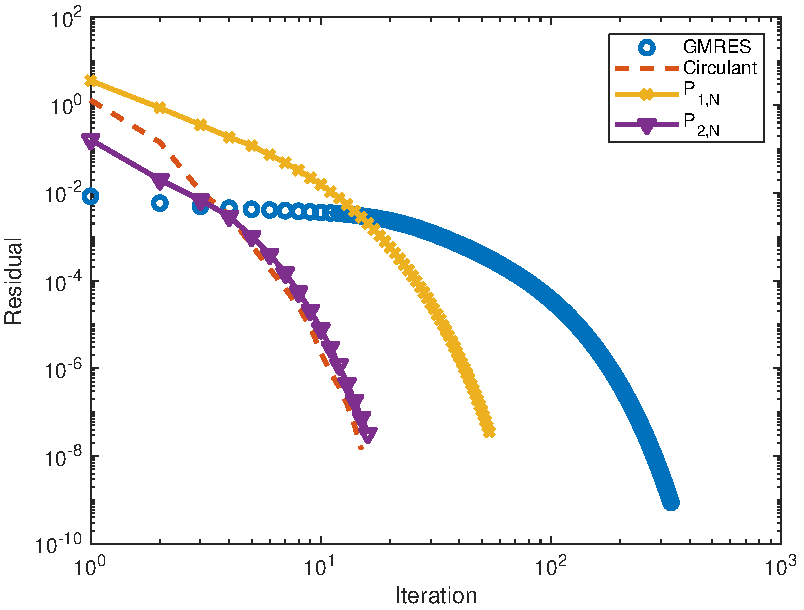
\includegraphics[width=\columnwidth]{gmresN=2048alpha=1.5_glt.pdf}}%
\only<5>{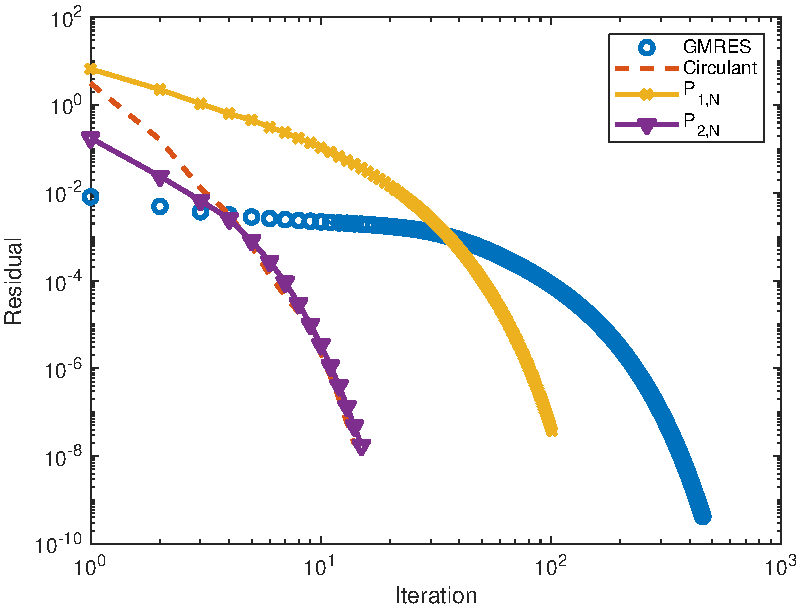
\includegraphics[width=\columnwidth]{gmresN=2048alpha=1.6_glt.pdf}}%
\only<6>{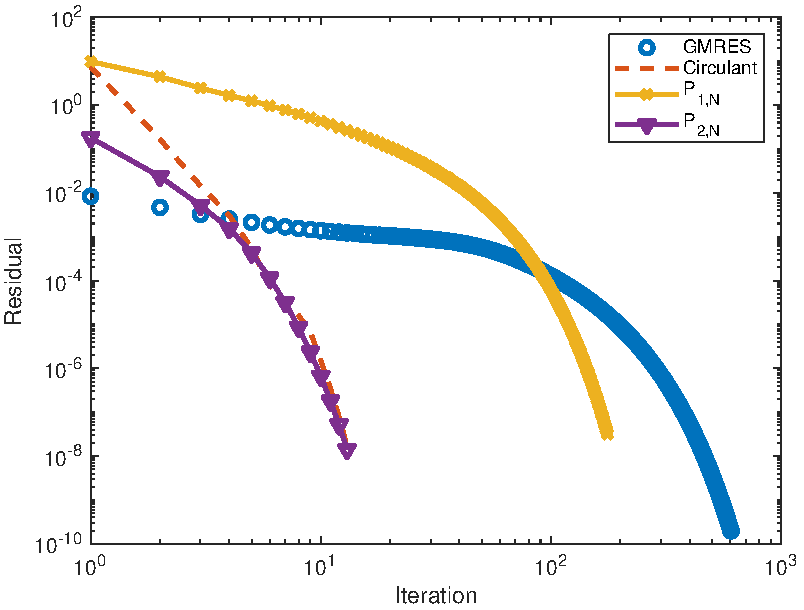
\includegraphics[width=\columnwidth]{gmresN=2048alpha=1.7_glt.pdf}}%
\only<7->{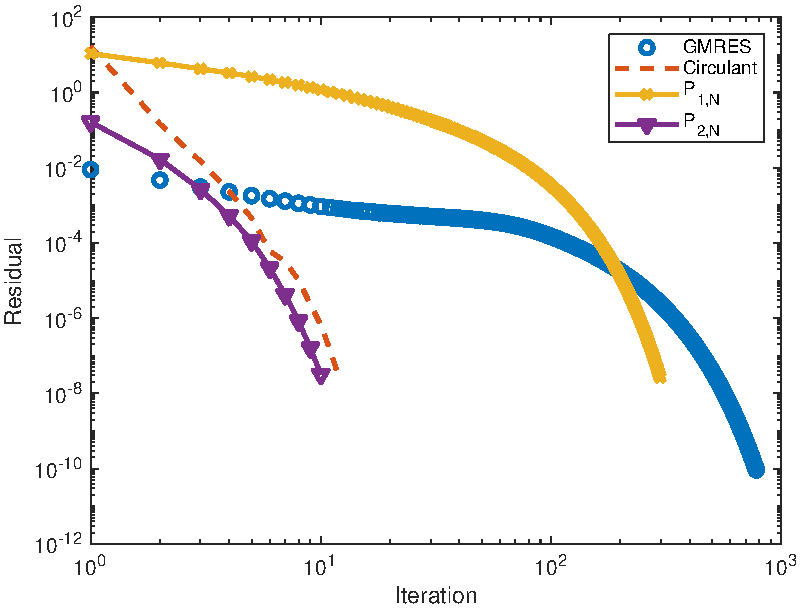
\includegraphics[width=\columnwidth]{gmresN=2048alpha=1.8_glt.pdf}}%
\end{column}
\end{columns}
\onslide<8->{\faHammer\;To \textbf{do better} we need to move towards Multigrid methods.}
\end{frame}

\subsection{Hints to the literature}

\begin{frame}{Circulant matrices at any cost}

Despite the \textbf{clear negative results} concerning the impossibility of obtaining a cluster using circulant matrices in the space-dependent case, the \emph{literature contains several attempts} in this direction.

\onslide<2->{One of the most reused idea originates from \parencite{MR3278848}, and goes as follows 
\begin{enumerate}
	\item<2-> We want to solve a ``diagonal times Toeplitz'' linear system, i.e.,
	\[
	A_N = \nu I_N - \left( D_N^+ G_N + D_N^- G_N^T \right),
	\]
	\item<3-> Call $d_i^+ = d^+(x_i)$ and $d_i^- = d(x_i)$, $i=1,2,\ldots,N$,
	\item<4-> Define the Toeplitz matrices
	\[
	K_i = \nu I_n - \left( d_i^+ G_N + d_i^- G_N^T \right), \qquad i=1,2,\ldots,N.
	\]
	\item<5-> Since $\mathbf{e}_i^T A_N = e_i^T K_i$, approximate
	\[
	\textbf{e}_i^T A^{-1} \approx \mathbf{e}_i^T K_i^{-1}.
	\]
\end{enumerate}
}

\end{frame}

\begin{frame}{Circulant matrices at any cost}\definecolor{amber}{rgb}{1.0, 0.75, 0.0}
But how do we approximate the inversion?
\begin{itemize}
	\item[\faLightbulb]<2-> Build $\displaystyle P_1 = \sum_{i=1}^{N} \mathbf{e}_i \mathbf{e}_i^T K_i^{-1}$ \onslide<3->{ \\\alert{\faSadTear}\;it costs too much! $N$ Toeplitz solve per iteration. }
	\item[\faLightbulb]<4-> Build $\displaystyle P_2 = \sum_{i=1}^{N} \mathbf{e}_i \mathbf{e}_i^T C_i^{-1}$ with $C_i = s(K_i)$ (Strang preconditioner) \onslide<5->{\\\alert{\faSadCry}\;it still cost too much! $O(N^2 \log(N))$ per iteration.}
	\item[\faLightbulb]<6-> Build $\displaystyle P_3 = \sum_{i=1}^{N} \mathbf{e}_i \mathbf{e}_i^T \sum_{j=1}^{\ell} \phi_j(x_i) C_j^{-1}$ \onslide<7->{ \textcolor{amber}{\faMeh}\; The cost is now $O(\ell N \log N)$ operations.} 
	\begin{itemize}
		\item[\faCog] where for $\ell \ll N$ values $\{x_{i_j}\}_{j=1}^{\ell} \subset \{x_i\}_{i=1}^{N}$ $\phi_j(x)$ are the basis of the piecewise linear interpolation of
		\[
		q_\lambda(x) = \frac{1}{\nu + \lambda d^+(x) + \overline{\lambda} d^-(x)}, \qquad \lambda \in \mathbb{C}.
		\]
	\end{itemize}
\end{itemize}
\end{frame}

\begin{frame}{Circulant matrices at any cost}\definecolor{amber}{rgb}{1.0, 0.75, 0.0}
The analysis of the \textcolor{amber}{\faMeh}\;$P_3$ preconditioner is quite involved, furthermore
\begin{itemize}
	\item[\faCogs] the iteration number dependence on the selection of the interpolation nodes and the value of $\lambda$ is unclear,
	\item[\faCogs] the \textbf{resulting preconditioner} is \textbf{always a circulant matrix}, thus the general theory tells us that there is \alert{no hope of} getting \alert{a cluster} of any sort.
\end{itemize}

\onslide<2->{\vfill\alert{\faExclamationTriangle}\; The extension of this preconditioners to the multi-dimensional settings is even more challenging: interpolation of surfaces, and higher dimensional objects is a tough problem!}

\onslide<3->{\vfill\alert{\faTimes}\; For these reasons we will not pursue further these results, if you are interested start from~\parencite{MR3278848}, and look to the next episodes.}

\end{frame}

	\section{Multidimensional cases}
	\only
	\begin{frame}{Multidimensional cases}
	What happens if our equation becomes
	\begin{equation*}
	\begin{cases}\frac{\partial W}{\partial t} = \left( \only<1>{\theta}\only<2>{d^+_x(x,t)}  \,{}^{\only<1->{RL}}D_{[0,x]}^\alpha  \cdot + \only<1>(1-\theta)\only<2>{d^-_x(x,t)} {}^{\only<1->{RL}}D_{[x,1]}^\alpha \cdot \right) W(x,y,t) + \only<1>{\qquad \theta \in [0,1]},\\
	\phantom{\frac{\partial W}{\partial t} =}\left( \only<1>{\theta}\only<2>{d^+_y(x,y,t)}  \,{}^{\only<1->{RL}}D_{[0,y]}^\alpha  \cdot + \only<1>(1-\theta)\only<2>{d^-_y(x,y,t)} {}^{\only<1->{RL}}D_{[y,1]}^\alpha \cdot \right) W(x,y,t)\\
		W(0,t) = W(1,t) = 0, \qquad W(x,t) = W_0(x).	
	\end{cases}
	\end{equation*}
	\begin{onlyenv}<1>
	\begin{itemize}
		\item[\faWrench] If we repeat the discretization procedure we have used in the 1D case we end up with a \textbf{block-Toeplitz-with-Toeplitz-blocks} matrix,
		\item[\faLightbulb] then we could attempt solution by using a \alert{block-circulant-with-circulant-blocks} preconditioner! In the 1D case (either symmetric or not) the procedure was working, maybe we are lucky$\ldots$
	\end{itemize}
	\end{onlyenv}
	\begin{onlyenv}<2>
	\begin{itemize}
		\item[\faWrench] It should not be difficult to imagine, but in this case we should end up again with a \textbf{matrix sequence of GLT type},
		\item[\faLightbulb] we can attempt the solution by doing something similar to what we have done in the 1D case: using a Toeplitz preconditioner$\ldots$
	\end{itemize}
	\end{onlyenv}

	\end{frame}

	\begin{frame}{\faSadTear\,A negative result}
		
	In the constant coefficient case we have a \textbf{general negative result}:
	\begin{quote}
		``Any Circulant-Like Preconditioner for Multilevel
		Matrices Is Not Superlinear'' -- \cite{MR1718339}
	\end{quote}

	\begin{alertblock}{Theorem \parencite[Theorem~4.1]{MR1718339}}
	For $I_n + A_n$, $A_n = A_n(f)$ a $p$-level Toeplitz matrix, any preconditioner for the form $I_n + C_n$, where $p_n$ is a $p$-level circulant matrix, is not superlinear.
	\end{alertblock}

	\begin{itemize}
		\item[\alert{\faBomb}]<2-> The \textbf{number of iterations} for the preconditioned system \textbf{will always depend on the size of the system}!
		\item[\faHammer]<3-> The dependence can still by milder than the one of the original system, thus there are cases in which this could be worthwhile (at least for a while).
	\end{itemize}\vspace{-0.5em}
	\begin{exampleblock}<4->{It is a difficult world}
	Already the case with constant coefficient is difficult to treat. Maybe we can find a way to \emph{reduce the number of dimensions}.
	\end{exampleblock}
	
	\end{frame}

	\begin{frame}{\faSadTear\,Another negative result and a proposal}
	\begin{itemize}
		\item[\alert{\faBomb}] The result we have obtained by means of GLT theory for the variable coefficient case remains valid also in two dimensions: \emph{no circulant preconditioner can have a strong cluster}!
		
		\item[\faLightbulb]<2-> We could attempt generalizing the $P_{1,N}$ and $P_{2,N}$ preconditioners to the new setting.
		
		\item[\faCogs]<3-> The matrix of the system in 2D has now the form
		\[
		A_\mathbf{N} = \nu I_\mathbf{N} - \left( D_\mathbf{N}^+ (G_{N_x} \otimes I_{N_y}) +  D_\mathbf{N}^- (I_{N_x} \otimes G_{N_y}) \right), \qquad \mathbf{N} = (N_x,N_y).
		\]
		\begin{itemize}\vspace{-1.5em}
			\item[\faDoorOpen]\normalsize If the \textbf{diffusion coefficients} are \textbf{constants}, this a BTTB matrix,
			\item[\faDoorOpen]\normalsize If the \textbf{diffusion coefficients} are \textbf{space variant}, we can show (following the same road as before) that the resulting matrix sequence is a GLT sequence.
		\end{itemize}
		\item[\faCogs]<4-> $P_{1,\mathbf{N}} = \nu I_\mathbf{N} -\left( D_\mathbf{N}^+ (T_{N_x}(1-e^{-i\theta_1}) \otimes I_{N_y}) +  D_\mathbf{N}^- (I_{N_x} \otimes T_{N_y}(1-e^{-i\theta_2})) \right)$; 
		\item[\faCogs]<4-> $P_{2,\mathbf{N}} = \nu I_\mathbf{N} -\left( D_\mathbf{N}^+ (T_{N_x}(2-2\cos(\theta_1)) \otimes I_{N_y}) +  D_\mathbf{N}^- (I_{N_x} \otimes T_{N_y}(2-2\cos(\theta_2)) \right)$.
	\end{itemize}

	\end{frame}

	\subsection{The structure preserving preconditioners}

	\begin{frame}{The structure preserving preconditioners}
	\faExclamationCircle\;To apply both $P_{1,\mathbf{N}}$ and $P_{2,\mathbf{N}}$ we now need to \textbf{solve an auxiliary sparse linear system} related to the \textbf{discretization of a 2D problem}.
	
	\begin{itemize}
		\item[\faHammer] Using a \alert{sparse direct solver} is not going to scale well with $\mathbf{N} = (N_x,N_y)$,
		\item[\faBomb]<2-> We need to \textbf{employ an iterative technique} to do the \textbf{preconditioner application}!
		\item[\faWrench]<3-> Methods of this type are usually called \textbf{multi-iterative methods}
		\begin{itemize}
			\item[$\Rightarrow$] \normalsize If we apply $P_{1,\mathbf{N}}$ or $P_{2,\mathbf{N}}$ using a fixed number of iterations of a fixed point technique, then we can still use GMRES,
			\item[$\Rightarrow$] \normalsize If we  apply $P_{1,\mathbf{N}}$ or $P_{2,\mathbf{N}}$ using a variable number of iterations of a fixed point technique or a \emph{nonstationary solver}, then we have to use the Flexible-GMRES.
		\end{itemize}
	\end{itemize}

	\begin{exampleblock}<4->{\faQuestionCircle\;What is the right combination?}
	The right combination of iterative schemes to use does really depend on the machine we have under our hands!
	\end{exampleblock}
	
	\end{frame}

	\subsection{Flexible-GMRES}

	\begin{frame}{Flexible-GMRES \parencite{MR1204241}}
		
	The \textbf{Flexible variant of GMRES} is built from the \emph{right-preconditioned} GMRES algorithm.
	
	\begin{columns}
	\begin{column}{0.5\columnwidth}\small
	\begin{algorithm}[H]
		\KwIn{$A \in \R^{n\times n}$, $m$, $\mathbf{x}^{(0)}$, $M \in \mathbb{R}^{n\times n}$}
		$\mathbf{r}^{(0)} \leftarrow b - A \mathbf{x}^{(0)}$\tcc*{Arnoldi process}
		$\beta \leftarrow \|\mathbf{r}^{(0)}\|_2$, 
		$\mathbf{v}^{(1)} \leftarrow \nicefrac{\mathbf{r}^{(0)}}{\beta}$\;
		\For{$j=1,\ldots,m$}{
			$\alert<2>{\mathbf{z}^{(j)}} \leftarrow P^{-1}\mathbf{v}^{(j)}$\;
			$\mathbf{w} \leftarrow A \mathbf{z}^{(j)}$\;
			\For{$i=1,\ldots,j$}{
				$h_{i,j} \leftarrow <\mathbf{w},\mathbf{v}^{(i)}>$\;
				$\mathbf{w} \leftarrow \mathbf{w} - h_{i,j} \mathbf{v}^{(i)}$\;
			}
			$h_{j+1,j} \leftarrow \|\mathbf{w}\|_2$\;
			$\mathbf{v}^{(j+1)} \leftarrow \nicefrac{\mathbf{w}}{h_{j+1,j}}$\;
		}
	\end{algorithm}
	\end{column}
	\begin{column}{0.5\columnwidth}
	\begin{algorithm}[H]\small
		\setcounter{AlgoLine}{12}
	\only<1>{\alert<1>{$V_m \leftarrow [\mathbf{v}^{(1)},\ldots,\mathbf{v}^{(m)}]$}}\only<2>{\alert<2>{$Z_m \leftarrow [\mathbf{z}^{(1)},\ldots,\mathbf{z}^{(m)}]$}}\;
	\tcp{Build the Krylov subspace basis}
	$\mathbf{y}^{(m)} \leftarrow \arg\min_{\mathbf{y}} \|\beta \mathbf{e}_1 - \overline{H}_m \mathbf{y}\|_2$\;
	\only<1>{\alert{$\mathbf{x}^{(m)} \leftarrow \mathbf{x}^{(0)} + P^{-1}V_m \mathbf{y}^{(m)}$}}\only<2>{\alert{$\mathbf{x}^{(m)} \leftarrow \mathbf{x}^{(0)} + Z_m \mathbf{y}^{(m)}$}}\;
	\tcp{Conv. check, possibly a restart}
	\eIf{ \emph{Stopping criteria satisfied} }{
		\textbf{Return:} $\tilde{\mathbf{x}} = \mathbf{x}^{(m)}$\;
	}{
		$\mathbf{x}^{(0)} \leftarrow \mathbf{x}^{(m)}$\tcc*{Restart}
		\textbf{goto} 1\;
	}
	\end{algorithm}
		
	\only<1>{\begin{alertblock}{\normalsize Same preconditioner}\small
	Line 15 forms the approximate
	solution of the linear system as $\mathbf{x}^{(0)} + P^{-1}V_m \mathbf{y}^{(m)}$.
	\end{alertblock}}
	\only<2>{\begin{alertblock}{\normalsize Changing preconditioner}\small
	Line 15 forms the approximate
	solution of the linear system as $\mathbf{x}^{(0)} + Z_m \mathbf{y}^{(m)}$.
		\end{alertblock}
	
	}

	\end{column}
	\end{columns}
	
	\end{frame}

	\begin{frame}{Flexible-GMRES \parencite{MR1204241}}
	With this variant of the GMRES we are solving
	\[
	A P^{-1} \mathbf{y} = \mathbf{b}, \text{ with } P\mathbf{x} = \mathbf{y},
	\]
	with a preconditioner $P$ whose action depends on the vector to which it is applied,
	\begin{itemize}
		\item[\faMoneyBill] in \textbf{terms of memory} we have to store two basis instead of one,
		\item[\faArrowDown] we use the \textbf{true residual} instead of the preconditioned one: \emph{the results are more reliable!}
	\end{itemize}

	\onslide<2>{
	Some \textbf{usual choices} of multi-iterative schemes are
	\begin{itemize}
		\item[\faWrench] Inner/Outer GMRES method: we fix a preconditioner $P$, solve the systems
		\[
		\mathbf{z}^{(j)} \leftarrow P^{-1} \mathbf{v}^{(j)},
		\]
		by a recursive call to GMRES;
		\item[\faWrench] A Multigrid algorithm in which some \emph{smoother} or \emph{coarse solver} is non stationary;
		\item[\faWrench] Non stationary polynomial preconditioners.
	\end{itemize}
	}

	\end{frame}

	\subsection{Exploiting the Kronecker structure}

	\begin{frame}{Exploiting the Kronecker structure}
	The \textbf{multidimensional case} has a \textbf{new structure} we can exploit: \textbf{Kronecker sums}!
	\only<1>{
	\[A_\mathbf{N} = \nu I_\mathbf{N} - \left( D_\mathbf{N}^+ (G_{N_x} \otimes I_{N_y}) +  D_\mathbf{N}^- (I_{N_x} \otimes G_{N_y}) \right), \qquad \mathbf{N} = (N_x,N_y).\]
	}
	\only<2-3>{
	\[A_\mathbf{N} = \nu I_{N_x} \otimes I_{N_y} - \left( D_\mathbf{N}^+ (G_{N_x} \otimes I_{N_y}) +  D_\mathbf{N}^- (I_{N_x} \otimes G_{N_y}) \right), \qquad \mathbf{N} = (N_x,N_y).\]
	}
	\only<4>{
	\[A_\mathbf{N} = \nu I_{N_x} \otimes I_{N_y} - \left( (D_\mathbf{1,N_x}^+ \otimes D_{2,N_y}^+) (G_{N_x} \otimes I_{N_y}) +  (D_\mathbf{1,N_x}^- \otimes D_{2,N_y}^-) (I_{N_x} \otimes G_{N_y}) \right) \]
	}
	\only<5->{
	\[\text{ Find }X \text{ s.t. } \nu X - D_{2,N_y}^+ X G_{N_x}^T D_{1,N_x}^+ - D_{2,N_y}^- G_{N_y} X D_{1,N_x}^- = B \]
	}
	\begin{itemize}
		\item<3->[\faCogs] If we assume \textbf{separable coefficients}, i.e.,
		\[
		d^+(x,y) = d^+_1(x)d^+_2(y), \quad d^-(x,y) = d^-_1(x)d^-_2(y).
		\]
		\item<4->[\faCogs] We write the solution vector $\mathbf{x}$ as a matrix $X$ such that $\mathbf{x} = \operatorname{vec}(X)$, where $\operatorname{vec}(\cdot)$ is the operation that stacks the columns of $X$, and the right-hand side $\mathbf{b}$ as $B$ with $\mathbf{b} = \operatorname{vec}(B)$.
		\item<5->[\faWrench] We got ourselves a \textbf{matrix equation} involving objects of ``smaller size''.
	\end{itemize}
	\end{frame}

\section{Conclusion and summary}

\begin{frame}{Conclusion and summary}
	\definecolor{success}{HTML}{4a934a}
	\definecolor{todo}{HTML}{0099cc}
	
	\begin{itemize}
		\item[\textcolor{success}{\faCheckCircle}] We have characterized the \textbf{spectral properties} of the involved matrix sequences,
		\item[\textcolor{success}{\faCheckCircle}] We investigated several preconditioning strategies that made use of the \textbf{structure} of the \textbf{underlying matrices},
		\item[\textcolor{success}{\faCheckCircle}] We started investigating \alert{multi-iterative schemes} and looking for ways of reducing the dimensionality of the involved problems.
	\end{itemize}

	Next up
	\begin{itemize}
		\item[\textcolor{todo}{\faClipboardList}] How and when do we solve the \textbf{matrix equation} formulation,
		\item[\textcolor{todo}{\faClipboardList}] What do we do when we have more than two dimensions?
		\item[\textcolor{todo}{\faClipboardList}] All-at-once formulations.
	\end{itemize}
		
	\end{frame}

	\section*{Bibliography}
	{\unnumbered
		\begin{frame}[allowframebreaks,noframenumbering]{Bibliography}
			\small
			\printbibliography
			
		\end{frame}
	}
\end{document}